% This file is part of the multi-tex ECE 486 Final Project Report 
% file name: report.tex

% YOU CAN COMPILE FROM THIS FILE, THIS IS THE MAIN FILE

\documentclass[12pt,a4paper,twoside]{report}
%\usepackage{mathptmx} %Times font
% Add these packages in preamble
\usepackage{multirow}
\usepackage[table]{xcolor}
\usepackage{float}
\usepackage{graphicx}
\usepackage{longtable}
\usepackage{float}
\usepackage{amsmath}
\usepackage[ruled,lined,linesnumbered]{algorithm2e}
\usepackage{amsfonts}
\usepackage{color}
\usepackage{amssymb}
\usepackage{graphicx}
\usepackage{chngcntr}
\usepackage{cite}
\usepackage{fancyhdr}
\usepackage[export]{adjustbox}
\usepackage{titlesec}
\usepackage{tabularx}
\usepackage{enumitem}
\usepackage{mathtools}
\usepackage[toc,page]{appendix}
\usepackage[normalem]{ulem}
\usepackage{booktabs}
\usepackage{rotating}
\usepackage{longtable}
\usepackage{caption}
\usepackage{pdflscape}
\usepackage [english]{babel}
\usepackage [autostyle, english = american]{csquotes}
\usepackage{listings}
\MakeOuterQuote{"}

\setlength{\voffset}{-0.75in}
\setlength{\headsep}{10pt}
\setlength{\parindent}{0cm}
\raggedbottom

\titlespacing{\section}{0pt}{0pt}{0pt}
\counterwithin{figure}{chapter}
\numberwithin{equation}{chapter}
\renewcommand{\baselinestretch}{1.2}
\renewcommand{\thetable}{\arabic{chapter}.\arabic{table}} 
\renewcommand{\footrulewidth}{0.4pt}
\textheight 245mm \textwidth 160mm \topmargin 15mm\setlength{\oddsidemargin}{.1in}
\evensidemargin .1in 
\titleformat{\chapter}[block]
{\normalfont\huge\bfseries}{\chaptertitlename\ \thechapter: }{0pt}{\huge}
\titlespacing*{\chapter}{0pt}{-20pt}{10pt}
\pagestyle{fancy}
\cfoot{}
\lhead{{\footnotesize EvoRAG: Evolutionary Multi-Personality RAG}}
\lfoot{Dept.of CSE, S.I.T.,Tumakuru-03}
\rfoot{\thepage}
\rhead{2025-26}
\linespread{1.5}
\numberwithin{equation}{chapter}
\let\cleardoublepage\clearpage
\bibliographystyle{unsrt}


\begin{document}
\addtocontents{toc}{\protect\thispagestyle{empty}}

\begin{titlepage}
\thispagestyle{empty}
 \centering
 {\textbf {SIDDAGANGA INSTITUTE OF TECHNOLOGY, TUMAKURU-572103}} \\
\textbf{{\small (An Autonomous Institute under Visvesvaraya Technological University, Belagavi)}}
	$$
\includegraphics[scale=1.0]{Logo}$$
\begin{center}
{\Large	 \textbf{Project Report (Phase-I) on}}\\[0.5cm]

{\color{black} {{\textbf {\Large \color{black} "EvoRAG: Evolutionary Multi-Personality RAG for Real-time Information Analysis"}}}} \\[0.5cm]
{{\large submitted in partial fulfillment for the completion of VI Semester }} \\
{ \textbf{\large	BACHELOR OF ENGINEERING\\	in\\	 COMPUTER SCIENCE \& ENGINEERING\\}} 
{\textbf {\large Submitted by}}\\[0.7cm]
	
\end{center}


\begin{center}
\textbf{Batch ID 12}\\
\begin{tabular}{ll}
Priyanka Kumari & (1SI23CS142)  \\
Shambhavi D C & (1SI23CS163)  \\
Sneha Kurane & (1SI23CS174)  \\
Tanushka Rani & (1SI23CS182)  \\
\end{tabular}\\[1.0cm]
\end{center}

\begin{center}
under the guidance of

\textbf{Dr. Sheela S}\\
Assistant Professor\\
Department of CSE\\
SIT, Tumakuru-03\\[1.0cm]
\end{center}


{\textbf{{{\small DEPARTMENT OF COMPUTER SCIENCE \& ENGINEERING \\2025-26}}}}

\end{titlepage}





\begin{titlepage}


\begin{center}
 {\textbf {SIDDAGANGA INSTITUTE OF TECHNOLOGY, TUMAKURU-572103}} \\
{ (An Autonomous Institute under Visvesvaraya Technological University, Belagavi)}
\textbf{{\small {DEPARTMENT OF COMPUTER SCIENCE \& ENGINEERING}}}
	$$
\includegraphics[scale=1.0]{Logo}$$

{\color{red}{\Large	\bf CERTIFICATE}}\\[0.5cm]
\end{center}

This is to certify that the project work entitled {\color{blue}"EVORAG: EVOLUTIONARY MULTI-PERSONALITY RAG FOR REAL-TIME INFORMATION ANALYSIS"} is a bonafide work carried out by Priyanka Kumari (1SI23CS142), Shambhavi DC (1SI23CS163), Sneha Kurane (1SI23CS174) and Tanushka Rani (1SI23CS182) in partial fulfillment for the the completion of VI semester Bachelor of Engineering in Computer Science \& Engineering from Siddaganga Institute of Technology, an autonomous institute under Visvesvaraya Technological University, Belagavi during the academic year 2025-26. It is certified that all corrections/suggestions indicated for internal assessment have been incorporated in the report submitted in the department library. The Project report has been approved as it satisfies the academic requirements in respect of project work prescribed for the Bachelor of Engineering degree.\\[1.0cm] 
	
\begin{tabular}{lll}
Dr.\ Sheela S    \hspace*{7cm} &     &        Dr. N R Sunitha \hspace{2cm}  \\
Assistant Professor   &   & Head of the Department          \\
Dept. of CSE   &  & Dept. of CSE        \\
SIT,Tumakuru-03     &  & SIT,Tumakuru-03             
\end{tabular}\\[1.0cm]


\textbf{External viva:}\\
\textbf{Names of the Examiners} \hspace{6.0cm} \textbf{Signature with date}\\
\textbf{1.}\\
\textbf{2.}\\

\end{titlepage}




\clearpage{\pagestyle{empty}\cleardoublepage}
\begin{titlepage}
\begin{center}
{\Large \textbf{ACKNOWLEDGEMENT}}
\end{center}

We offer our humble pranams at the lotus feet of \textbf{His} Holiness, \textbf{Dr. Sree Sree Sivakumara Swamigalu}, Founder President and \textbf{His} Holiness, \textbf{Sree Sree Siddalinga Swamigalu}, President, Sree Siddaganga Education Society, Sree Siddaganga Math for bestowing upon their blessings.\\

We deem it as a privilege to thank \textbf{Dr. Shivakumaraiah}, CEO, SIT, Tumakuru,  and \textbf{Dr. S V Dinesh}, Principal, SIT, Tumakuru for fostering an excellent academic environment in this institution, which made this endeavor fruitful.\\

We would like to express our sincere gratitude to \textbf{Dr. N R Sunitha}, Professor and Head, Department of CS\&E, SIT, Tumakuru for her encouragement and valuable suggestions.\\

We thank our guide \textbf{Dr. Sheela S, Assistant Professor},  Department of Computer Science \& Engineering, SIT, Tumakuru for the valuable guidance, advice and encouragement.\\


\begin{flushright}
\begin{tabular}{ll}
Priyanka Kumari & (1SI23CS142)  \\
Shambhavi D C & (1SI23CS163)  \\
Sneha Kurane & (1SI23CS174)  \\
Tanushka Rani & (1SI23CS182)  \\
\end{tabular}\\[1.5cm]
\end{flushright}
\end{titlepage}
\begin{titlepage}
\begin{center}
{\Large \textbf{Course Outcomes}}
\end{center}
After successful completion of major project, graduates will be able:\\
CO1: To identify a problem through literature survey and knowledge of contemporary engineering technology. \\      
	% PO12: Life  long learning (3)\\
CO2: To consolidate the literature search to identify issues/gaps and formulate the engineering problem \\
%PO2  Problem analysis(3)\\
CO3: To prepare project schedule for the identified design methodology and engage in budget analysis, and share responsibility for every member in the team\\
%PO11  Project management and finance (3)\\
CO4: To provide sustainable  engineering solution considering health, safety, legal, cultural issues and also demonstrate concern for environment \\
%PO6 Engineer and Society (3)\\
%PO7 Environment and sustainability (3)\\
CO5: To identify and apply the mathematical concepts, science concepts, engineering and management concepts necessary to implement the identified engineering problem \\
%PO1 Engineering Knowledge \\
%PO2 Problem Analysis(3)
CO6: To select the engineering tools/components required to implement the proposed solution for the identified engineering problem\\
%PO5 Modern tool Usage(3) \\
CO7: To analyze, design, and implement optimal design solution, interpret results of  experiments and draw valid conclusion \\
%PO3 Design/Development of Solutions(3) \\
%PO4 Conduct investigation of complex problems(3)\\
CO8: To demonstrate effective written communication through the project report, the one-page poster presentation, and preparation of the video about the project and the four page IEEE/Springer/ paper format of the work\\
%PO10 Communication (3)\\
CO9: To engage in effective oral communication through power point presentation and demonstration of the project work\\ 
%PO10 Communication(3)\\
CO10:To demonstrate compliance to the prescribed standards/ safety norms and abide by the norms of professional ethics\\
%PO8 Ethics(3)\\
CO11: To perform in the team, contribute to the team and mentor/lead the team
%PO9 Individual and Team work (3)\\
\newpage
\begin{table}[ht]
\caption*{\textbf{CO-PO Mapping}}
\resizebox{\textwidth}{!}{%
\begin{tabular}{|l|l|l|l|l|l|l|l|l|l|l|l|l|l|l|}
\hline
 & PO1 & PO2 & PO3 & PO4 & PO5 & PO6 & PO7 & PO8 & PO9 & PO10 & PO11 &  PSO1 & PSO2 &PSO3 \\ \hline
CO-1 &  &  &  &  &  &  &  &  &  &  &  3 & 3 &  \* &  \ \\ \hline
CO-2 &  & 3 &  &  &  &  &  &  &  &  &    &  &  &  \\ \hline
CO-3 &  &  &  &  &  &  &  &  &  & 3 &   &  &  &  \\ \hline
CO-4 &  &  &  &  &  & 3 &  &  &  &  &    &  & 3 & 3 \\ \hline
CO-5 & 3 & 3 &  &  &  &  &  &  &  & &   &  & 3 &  \\ \hline
CO-6 &  &  &  &  & 3 &  &  &  &  &  &  3  &  &3  &  \\ \hline
CO-7 &  &  & 3 & 3 &  &  &  &  &  &  &    &3 &3  &3  \\ \hline
CO-8 &  &  &  &  &  &  &  &  & 3 &  &    &  & &  \\ \hline
CO-9 &  &  &  &  &  &  &  &  & 3 &  &    &  & &  \\ \hline
CO-10 &  &  &  &  &  &  & 3 &  &  &  &    &  &  &  \\ \hline
CO-11 &  &  &  &  &  &  &  & 3 &  &  &   &  &  &  \\ \hline

Average & 3 & 3 & 3 & 3 & 3 & 3 & 3 & 3 & 3 & 3 & 3  &  & &\\ \hline
\end{tabular}%
}
\end{table}
$\*$ Attainment level: \\ 1: Slight (low) 2: Moderate (medium) 3: Substantial (high)
\\ \\POs: \\ PO1: Engineering knowledge,\\ PO2: Problem analysis,\\ PO3:Design of solutions, \\PO4:Conduct investigations of complex problems,
\\PO5: Engineering tool usage,\\ PO6:Engineer and the world,\\ PO7:Ethics, \\PO8:Individual and collaborative work,\\ PO9:communication, 
\\PO10:project management and finance,\\PO11: Life-long learning.
\\ PSOs
\\ PSO1: Computer based systems development
\\	PSO2: Software development
\\ PSO3: Computer communications and Internet applications

\end{titlepage}
%\input{ProjectEvaluationRubrics}
\pagenumbering{roman}
\chapter*{Abstract}
\thispagestyle{plain}
\addcontentsline{toc}{chapter}{\numberline{}Abstract}

Large Language Models (LLMs) have become central to modern information retrieval.Despite their capabilities, LLMs are constrained by static training data and lack access to current or domain-specific knowledge. Retrieval-Augmented Generation (RAG) was introduced to address this limitation by enabling models to retrieve and incorporate external information at inference time. However, existing RAG systems follow a linear, single-pass pipeline that generates one response without exploring alternative interpretations or verifying factual accuracy. This results in outputs that are often one-sided, prone to hallucination, and lacking analytical depth.

This project proposes \textbf{EvoRAG (Evolutionary Multi-Persona RAG)}, a framework designed to improve the quality and reliability of AI-generated responses through structured multi-perspective reasoning. EvoRAG orchestrates eight distinct AI personas, each representing a different reasoning style, to analyze the same retrieved context simultaneously. Responses are evaluated through an internal consensus mechanism that scores outputs based on factual accuracy, analytical depth, and clarity, ensuring the final answer reflects collective reasoning rather than a single viewpoint.

The system includes an \textbf{Evolutionary Learning Engine} that tracks persona performance over time using internal win rates and user feedback, autonomously replacing underperforming agents with improved variants. Additionally, EvoRAG operates entirely on local hardware, eliminating dependence on external APIs and ensuring that sensitive user data remains private.

The expected outcome is a significant reduction in AI hallucinations and a measurable improvement in response quality compared to standard RAG architectures, achieved through cognitive diversity, iterative refinement, and privacy-preserving local deployment.
\tableofcontents
\thispagestyle{empty}
\pagenumbering{roman}
\listoffigures
\addcontentsline{toc}{chapter}{\numberline{}List of Figures}

\listoftables
\addcontentsline{toc}{chapter}{\numberline{}List of Tables}

\cleardoublepage

\pagenumbering{arabic}
\setcounter{page}{1}
\chapter{Introduction}

Large Language Models (LLMs) have transformed the field of natural
language processing, enabling computational systems to generate coherent, contextually
relevant responses across a wide range of tasks.
However, LLMs are constrained by a fundamental limitation: their knowledge is fixed
at the point of training.
When queried on topics beyond this boundary, models frequently produce responses that
are factually incorrect, a behaviour commonly referred to as
hallucination.

Retrieval-Augmented Generation (RAG) was introduced to mitigate this limitation by
enabling models to retrieve relevant information from external sources before generating
a response.
This approach grounds model outputs in real-world data and reduces reliance on static
parametric knowledge.
Subsequent work extended this paradigm further — first by demonstrating that fusing
multiple retrieved passages yields measurable gains on open-domain question
answering, and then by integrating retrieval directly into the pre-training stage,
producing representations that are inherently more
knowledge-aware.

Despite these advances, standard RAG implementations operate through a linear,
single-pass pipeline that retrieves a document, reads it once, and produces a single
response.
This design assumes a single valid interpretation of the retrieved content, which is
insufficient for complex analytical tasks that require critical evaluation,
cross-verification, or multi-perspective reasoning.
Efforts to address this limitation have led to frameworks that interleave retrieval
with iterative reasoning, and to self-reflective generation
mechanisms that allow a model to evaluate the quality of both its retrieved evidence
and its generated output before producing a final answer.

In addition, most high-performance RAG systems depend on cloud-based infrastructure,
requiring user queries and potentially sensitive data to be transmitted to external
servers.
This raises significant concerns regarding data privacy and sovereignty, particularly
in professional, medical, or research contexts where confidentiality is
essential.
Furthermore, existing systems are largely static; they do not adapt based on past
interactions or evolving user requirements, making repeated errors likely and limiting
their long-term utility.

To address these limitations, this project proposes \textbf{EvoRAG (Evolutionary
Multi-Persona RAG)}, a locally deployed, multi-agent framework that enhances
retrieval-augmented generation through structured cognitive
diversity.
EvoRAG orchestrates eight distinct AI personas, each with a different reasoning style,
to analyse retrieved content simultaneously and independently.
Their outputs are evaluated through an internal consensus mechanism that scores
responses based on factual accuracy, analytical depth, and clarity.
The system further incorporates an \emph{Evolutionary Learning Engine} that monitors
persona performance over time and autonomously replaces underperforming agents with
improved variants, based on internal win rates and user feedback.
All processing is performed on local hardware, ensuring that no user data is transmitted
externally.

% ------------------------------------------------------------------
\section{Motivation}

The decision to undertake EvoRAG as a project was driven by a confluence of
real-world observations and unresolved technical gaps in the current landscape of
AI-driven information systems.
As large language models became embedded in decision-making across healthcare, education,
legal services, and public discourse, a clear pattern emerged: these systems are capable
of generating highly confident yet factually incorrect responses, a behaviour with direct
consequences for anyone relying on them.
Witnessing the gap between the trust users place in AI-generated answers and the actual
reliability of those answers made it evident that the existing single-pass retrieval and
generation paradigm was insufficient for high-stakes analytical tasks.

A further motivating observation was the structural incompatibility of cloud-dependent
RAG deployments with privacy-sensitive domains.
In fields such as clinical medicine, legal practice, and enterprise research, routing
queries through external servers is not merely inconvenient — it may constitute a
direct regulatory violation.
The absence of a capable, locally deployable alternative that could match the analytical
depth of hosted systems represented a concrete and pressing gap that this project
is designed to fill.

The project was also motivated by the absence of any mechanism for transparency and
explainability in how existing RAG systems arrive at their responses.
A single answer, produced by a single reasoning trajectory, provides no insight into
what alternative interpretations were considered or rejected.
For users in professional contexts, this opacity undermines trust and limits
accountability.
EvoRAG was conceived to address this by making the diversity of reasoning visible —
eight independent personas each produce an analytical response before a consensus
is formed, giving users a richer and more auditable view of the reasoning process.

On the technical side, the specific limitations of existing RAG architectures provided
equally compelling motivation.
Standard pipelines retrieve a document, process it once, and emit a single output with
no internal mechanism to challenge, verify, or cross-validate the result.
Recent work on retrieval-interleaved reasoning and self-reflective generation has
shown the value of iterative evaluation, yet
these advances have not been integrated into a unified, locally deployable,
consensus-driven framework.
Furthermore, all deployed RAG systems observed during the course of this project shared
a common architectural flaw: they do not improve over time.
Query history, user feedback, and observed performance outcomes are discarded after
each session, making systematic error correction impossible without manual retraining.
This motivated the design of EvoRAG's evolutionary learning engine, which autonomously
refines persona configurations based on empirical win rates and accumulated feedback,
enabling the system to become more effective the longer it is used.

% ------------------------------------------------------------------
\section{Objectives of the Project}
% ------------------------------------------------------------------

The primary goals of the EvoRAG project are:

\begin{itemize}
    \item To build a robust pipeline that can autonomously retrieve and index external
          knowledge for local use at runtime, in direct response to each user query.
    \item To design a multi-agent framework that simulates eight distinct AI personas
          to provide diverse, parallel analytical views of the same retrieved context.
    \item To implement a peer-review scoring system that programmatically filters out
          weak or inaccurate responses through a structured consensus mechanism.
    \item To develop an evolutionary tracking system that improves the system's
          reasoning capability over time based on win rates and user feedback, without
          manual reconfiguration or retraining of the base model.
    \item To ensure all operations are local and privacy-preserving, removing the
          dependency on external APIs or cloud-based services entirely.
\end{itemize}

\section{Organisation of the Report}

This report is structured to provide comprehensive coverage of the proposed system's
design and implementation. The content is organised across five chapters as follows:

\begin{itemize}
    \item \textbf{Chapter 1: Introduction} — Presents the background, motivation, and
          objectives of the EvoRAG project, establishing the research context and the
          limitations of existing RAG systems that this work seeks to address.

    \item \textbf{Chapter 2: Literature Survey} — Surveys the relevant literature
          across agentic RAG frameworks, multi-agent collaboration, memory management,
          and evaluation methodology, and identifies the specific research gaps that
          EvoRAG is designed to address.

    \item \textbf{Chapter 3: System Overview} — Describes the functional and
          non-functional requirements of the system alongside the hardware, software,
          and overall architectural design of the proposed solution.

    \item \textbf{Chapter 4: Methodology} — Details the implementation approach,
          covering dataset preparation, knowledge ingestion, and the algorithmic
          operation of each core engine within the EvoRAG pipeline.

    \item \textbf{Chapter 5: Conclusion} — Presents the overall conclusions of the
          project, reflects on current limitations of the implemented system, and
          outlines directions for future research and development.
\end{itemize}
% ------------------------------------------------------------------
%  CHAPTER 2 – LITERATURE SURVEY
% ------------------------------------------------------------------
\chapter{Literature Survey}
 
This chapter provides a comprehensive review of recent advancements in
Retrieval-Augmented Generation (RAG) and intelligent agent frameworks.
The field has progressed considerably from static knowledge retrieval toward dynamic,
corrective, and agentic systems that aim to minimise hallucinations and improve reasoning
depth across a variety of knowledge-intensive tasks.
The survey is structured to trace this progression from foundational contributions
through to the most recent advances in agentic orchestration, memory management,
hallucination mitigation, knowledge-graph integration, and hierarchical retrieval,
culminating in an identification of the research gaps that EvoRAG is specifically
designed to address.

The foundational concepts behind EvoRAG are grounded in the original RAG
framework~\cite{lewis2020rag} and the retrieval-aware reasoning advances exemplified
by ReAct~\cite{yao2022react}.
Work on tool-oriented model orchestration in Toolformer~\cite{schick2023toolformer}
and the self-reflective generation architecture of Self-RAG~\cite{asai2023selfrag}
also directly influence the way EvoRAG integrates external knowledge and internal
consensus validation.
The broader context for these contributions is provided by the foundational study of
large-scale pre-trained language models as general-purpose systems~\cite{bommasani2021foundation},
which established the conceptual framework within which all subsequent retrieval
augmentation research is situated.
 
% ------------------------------------------------------------------
\section{Agentic RAG Frameworks}
% ------------------------------------------------------------------
 
The shift from traditional RAG pipelines to agentic architectures represents one of
the most significant developments in the field over the past two years.
Singh et al.~\cite{singh2025agenticrag} provide a comprehensive survey of Agentic RAG
systems, introducing a principled taxonomy of architectures classified by agent
cardinality, control structure, autonomy, and knowledge representation.
Their analysis demonstrates how embedding autonomous agents into the RAG pipeline
enables dynamic retrieval strategy management, iterative context refinement, and
multi-step reasoning that static, single-pass workflows are fundamentally unable to
achieve.
A key insight from this survey is that no single retrieval granularity is universally
optimal; effective agentic systems must be capable of dynamically selecting between
keyword, semantic, and document-level retrieval depending on the information density
of the query.
 
Complementing this taxonomic perspective, Du et al.~\cite{du2026arag} introduce
A-RAG, a hierarchical retrieval interface framework that exposes keyword search,
semantic search, and chunk-level read tools directly to the language model.
By granting the model the capacity to adaptively navigate across multiple retrieval
granularities, A-RAG consistently outperforms prior approaches while maintaining
comparable or lower retrieved token counts — demonstrating that architectural
flexibility can compensate for brute-force context scaling.
This finding is particularly relevant to EvoRAG's retrieval module, which similarly
distinguishes between coarse topic retrieval and fine-grained passage extraction
depending on the complexity of the query issued by each active persona.
 
More recently, the growing intersection of agentic retrieval and deep reasoning has
been surveyed by Li et al.~\cite{li2025ragreas}, who introduce a unified
Reasoning-Retrieval perspective that categorises methods along two complementary
axes: \emph{Reasoning-Enhanced RAG}, in which advanced reasoning optimises
individual stages of the retrieval pipeline; and \emph{RAG-Enhanced Reasoning}, in
which retrieved knowledge provides the missing factual premises required for complex
multi-step inference.
Their survey further identifies emerging \emph{Synergised RAG-Reasoning} frameworks,
where agentic LLMs iteratively interleave search and reflection to achieve
state-of-the-art performance on knowledge-intensive benchmarks — a paradigm that
directly informs the EvoRAG design.
The survey's emphasis on the mutual dependence of retrieval quality and reasoning
quality underlines why EvoRAG's personas are each assigned a distinct reasoning
style rather than simply sharing a common prompt template.

% ------------------------------------------------------------------
\section{Hierarchical and Graph-Based Retrieval Architectures}
% ------------------------------------------------------------------

A significant limitation of flat chunk-based retrieval is its inability to capture
the hierarchical and relational structure present in real-world document corpora.
Two complementary research directions have emerged to address this: recursive
abstractive retrieval and graph-based retrieval.

Sarthi et al.~\cite{sarthi2024raptor} introduce RAPTOR (Recursive Abstractive
Processing for Tree-Organized Retrieval), a framework that recursively clusters
and summarises retrieved text chunks into progressively higher-level abstractions,
constructing a tree structure over the document corpus.
At query time, retrieval can proceed at any level of the tree, enabling the system
to match coarse thematic queries against high-level summaries while still supporting
fine-grained factual lookups at the leaf level.
RAPTOR demonstrates substantial gains over flat retrieval baselines on multi-step
reasoning tasks, confirming that structural organisation of the retrieval index
yields qualitative improvements in answer coherence.
This hierarchical indexing principle informs EvoRAG's approach to knowledge base
construction, wherein retrieved passages are organised by topic cluster before
being distributed to individual personas.

Edge et al.~\cite{edge2024graphrag} extend the retrieval paradigm further by
proposing GraphRAG, a system that pre-constructs a community-structured knowledge
graph from an input corpus and uses this graph to answer global, query-focused
summarisation tasks.
By traversing the graph at the community level rather than retrieving isolated
passages, GraphRAG captures cross-document relationships and thematic patterns
that are entirely invisible to conventional vector-search retrieval.
The practical implication is that for analytical queries requiring synthesis across
many documents — precisely the class of queries for which EvoRAG is designed —
graph-structured retrieval provides qualitatively richer context than passage-level
retrieval alone.

The challenge of integrating structured knowledge from knowledge graphs with the
generative capabilities of LLMs is surveyed comprehensively by
Pan et al.~\cite{pan2024unifying}, who identify three principal integration
strategies: using LLMs to enhance knowledge graph construction, using knowledge
graphs to constrain LLM generation, and jointly training models over both text and
graph-structured data.
Their analysis highlights that hybrid retrieval — grounding generation in both
unstructured text and structured relational knowledge — consistently outperforms
either modality in isolation, particularly for queries involving entity-level
factual precision.
EvoRAG's architecture acknowledges this finding by designing the retrieval layer
to be modality-agnostic, capable of ingesting both plain text documents and
structured data formats.

% ------------------------------------------------------------------
\section{Hallucination Detection and Reliability in RAG Systems}
% ------------------------------------------------------------------

The tendency of large language models to produce factually incorrect yet
linguistically fluent outputs — a phenomenon widely referred to as hallucination —
represents the primary reliability challenge in deploying LLM-based systems for
high-stakes analytical tasks.
Manakul et al.~\cite{manakul2023selfcheckgpt} introduce SelfCheckGPT, a zero-resource
black-box hallucination detection method that exploits the statistical consistency
of multiple stochastic samples from the same model.
The core insight is that factual claims in a model's output will be consistently
reproduced across independently sampled responses if and only if those claims are
supported by strong parametric knowledge; hallucinated content, by contrast, tends
to vary inconsistently across samples.
SelfCheckGPT achieves state-of-the-art hallucination detection on the WikiBio
benchmark without requiring any reference documents or model internals, making it
directly applicable to black-box deployment scenarios.
This self-consistency principle is directly operationalised in EvoRAG's peer-review
scoring mechanism, where claims that appear consistently across multiple independently
generated persona responses receive higher consensus confidence scores.

Mallen et al.~\cite{mallen2023trust} investigate the conditions under which language
models should be trusted to answer from parametric memory versus those in which
external retrieval is essential.
Their study demonstrates that model confidence is a poor predictor of factual
accuracy for long-tail or temporally sensitive entities, motivating the need for
always-on retrieval rather than retrieval triggered only on model uncertainty signals.
This finding provides empirical justification for EvoRAG's unconditional retrieval
strategy, in which all queries are routed through the knowledge ingestion pipeline
regardless of perceived difficulty, ensuring that no query relies solely on
potentially stale parametric knowledge.

Shi et al.~\cite{shi2023replug} address the complementary problem of augmenting
black-box language models — those whose parameters cannot be modified — with a
retrieval component, through REPLUG (Retrieve and Plug).
REPLUG treats the language model as a scoring function and retrieves documents
whose prepending to the context maximises the model's likelihood on the query,
without any gradient-based fine-tuning of the underlying model.
This plug-and-play design philosophy is directly relevant to EvoRAG's architecture,
which runs retrieval-augmented generation over a locally deployed model whose
weights remain fixed, with adaptation achieved entirely through the evolutionary
persona configuration layer rather than through model retraining.

% ------------------------------------------------------------------
\section{Multi-Agent Collaboration in RAG}
% ------------------------------------------------------------------
 
Multi-agent collaboration has emerged as a particularly productive direction for
handling complex, ambiguous information-seeking tasks that exceed the capacity of any
single-agent pipeline.
Nguyen et al.~\cite{nguyen2025marag} present MA-RAG, a training-free multi-agent
framework that orchestrates four specialised agents — a Planner, a Step Definer, an
Extractor, and a QA Agent — to decompose queries into subtasks including query
disambiguation, evidence extraction, and answer synthesis.
By enabling agents to communicate via chain-of-thought reasoning, MA-RAG achieves
improved accuracy and interpretability on multi-hop and ambiguous question-answering
benchmarks without any model fine-tuning.
The framework's design makes explicit what has long been implicit in multi-step
retrieval pipelines: that different sub-tasks within a complex query require
qualitatively different reasoning strategies, and that separating these strategies
into distinct agents yields more reliable outcomes than conflating them within a
single prompt.
 
The problem of heterogeneous retrieval across structured and unstructured data sources
is addressed by Xiao et al.~\cite{xiao2026massrag}, who propose MASS-RAG, a
Multi-Agent Synthesis approach that assigns distinct roles to separate evidence
summarisation, evidence extraction, and reasoning agents.
By combining their intermediate outputs through a dedicated synthesis stage,
MASS-RAG exposes multiple complementary evidence views before committing to a final
answer, yielding consistent performance improvements over strong single-agent baselines.
Xu et al.~\cite{xu2026anchorrag} address the related challenge of open-world
knowledge graph traversal through AnchorRAG, a framework in which a supervisor agent
formulates iterative retrieval strategies for subordinate retriever agents, which
conduct parallel graph traversal before synthesising the resulting knowledge paths.
This hierarchical delegation strategy improves retrieval robustness and substantially
mitigates the impact of ambiguous or erroneous anchor entities, establishing new
state-of-the-art results on real-world multi-hop reasoning tasks.

The collective insight from these multi-agent frameworks is that the decomposition
of retrieval, reasoning, and synthesis into separate agents controlled by a
coordinator — whether heuristic or learned — is a broadly effective design pattern.
EvoRAG differs from this pattern not in its use of multiple agents but in the
nature of their interaction: rather than specialising each agent by function, EvoRAG
specialises agents by reasoning \emph{style}, allowing the same retrieval context
to be interpreted through distinct analytical lenses before a consensus is formed.

% ------------------------------------------------------------------
\section{Training and Traceability in Agentic RAG}
% ------------------------------------------------------------------
 
End-to-end training of agentic RAG systems using reinforcement learning has shown
strong promise for improving both retrieval reliability and reasoning traceability.
Zheng et al.~\cite{zheng2025deepdx} introduce Deep-DxSearch, an agentic RAG system
trained via reinforcement learning over a corpus of disease profiles, patient records,
and biomedical documents.
By co-optimising retrieval and reasoning through soft verifiable rewards, the system
learns to formulate queries, evaluate evidence, and iteratively refine searches —
directly addressing the disconnect from evidence-based reasoning that is endemic to
static RAG pipelines.
The medical domain context of this work is instructive: it demonstrates that
end-to-end RL training can instil traceable, evidence-grounded reasoning behaviours
even in the absence of direct supervision on intermediate reasoning steps.

The use of human preference signals to align language model behaviour more broadly
was established by Ouyang et al.~\cite{ouyang2022rlhf}, whose InstructGPT system
demonstrated that fine-tuning a language model via reinforcement learning from human
feedback (RLHF) produces outputs that are substantially more aligned with user intent
than those produced by a purely instruction-tuned model of the same scale.
The principle that empirical feedback from evaluators can be used to guide model
behaviour without retraining its core parameters is directly echoed in EvoRAG's
evolutionary engine, which treats user feedback and peer-review win rates as a
lightweight form of preference signal used to promote or demote individual persona
configurations.

% ------------------------------------------------------------------
\section{Data Synthesis for Robust RAG Agents}
% ------------------------------------------------------------------
 
A critical bottleneck in developing robust agentic RAG systems is the scarcity of
high-quality training data that faithfully reflects the retrieval noise encountered in
real-world deployments.
Addressing this gap, RAGShaper~\cite{anonymous2026ragshaper} introduces an automated
data synthesis framework that constructs dense information trees enriched with
adversarial distractor documents.
A constrained navigation strategy forces a teacher agent to actively confront these
distractors during trajectory generation, eliciting demonstrations that explicitly
model error correction and noise rejection.
Models trained on these synthetic trajectories significantly outperform baselines that
train on clean corpora, indicating that controlled adversarial exposure is a viable and
scalable path to improving agent robustness.

The closely related problem of enabling few-shot generalisation in retrieval-augmented
models is addressed by Izacard et al.~\cite{izacard2022atlas}, who introduce Atlas,
a pre-trained retrieval-augmented language model that achieves strong few-shot
performance on knowledge-intensive tasks by jointly training the retriever and the
reader end-to-end.
Atlas demonstrates that a model with access to a large, up-to-date retrieval index
can match or outperform models with orders-of-magnitude more parameters on factual
tasks, provided that the retriever and reader are trained in coordination.
This result motivates EvoRAG's emphasis on tight coupling between the retrieval
pipeline and the persona reasoning layer, rather than treating retrieval as a
preprocessing step decoupled from generation.
 
% ------------------------------------------------------------------
\section{Memory and Long-Term Knowledge in AI Agents}
% ------------------------------------------------------------------
 
Memory management is increasingly recognised as a foundational capability for
intelligent agents operating in complex, multi-session environments.
Hu et al.~\cite{hu2025memory} provide a comprehensive landscape of agent memory
research, proposing a unified taxonomy structured along three axes:
\emph{forms} (token-level, parametric, and latent memory);
\emph{functions} (factual, experiential, and working memory); and
\emph{dynamics} (formation, evolution, and retrieval).
This taxonomy moves beyond the conventional long-term versus short-term dichotomy and
establishes that agent failures are often rooted in deficiencies in memory dynamics
rather than model capacity alone — a finding with direct implications for the EvoRAG
evolutionary learning engine.
 
Complementing this taxonomic foundation, the challenge of \emph{joint} long-term and
short-term memory management has been formalised by
Chen et al.~\cite{chen2026agemem}, who propose AgeMem, a reinforcement learning-based
framework in which an agent learns autonomous policies for promoting, consolidating,
and retrieving information across memory tiers.
Their experiments demonstrate that an RL-trained agent substantially outperforms
heuristic-based memory management strategies on both embodied reasoning and
knowledge-intensive question-answering tasks, underscoring the practical value of
learning-based memory governance.
 
A further dimension of memory research, focused specifically on personalised
conversational continuity, is explored in the Memory OS of AI Agents
framework~\cite{bai2025memos}, which introduces a segmented paging architecture
for dialogue-chain memory.
The system partitions memory into active, inactive, and archival tiers governed by
heat-based mechanisms that model the temporal importance decay of stored episodes.
This operating-system-inspired abstraction enables contextual coherence and
personalised recall across extended, multi-session interactions — a capability that
EvoRAG's user adaptation module is designed to approximate through per-persona
affinity modelling.
The analogy between operating-system memory management and agent knowledge retention
is particularly apt: just as an OS must balance fast access to recently used pages
with long-term persistence of infrequently accessed data, EvoRAG must balance
responsiveness to recent user preferences with the cumulative evolutionary history
that determines which personas have demonstrated sustained analytical value.
 
% ------------------------------------------------------------------
\section{Comparative Evaluation of RAG Approaches}
% ------------------------------------------------------------------
 
As RAG systems grow in architectural complexity, systematic and reproducible evaluation
becomes increasingly critical for guiding practical deployment decisions.
Besrour et al.~\cite{besrour2026agenticvsenh} conduct an experiment-driven comparison
between Enhanced RAG and Agentic RAG across multiple domains, examining the impact of
LLM quality on system robustness and identifying the practical performance trade-offs
between fixed pipeline and agentic orchestration approaches.
Their findings provide actionable guidance for practitioners choosing between the two
paradigms and confirm that agentic orchestration offers measurable advantages on
multi-hop and reasoning-intensive queries, but that this advantage diminishes when
the underlying LLM quality is insufficient to support reliable tool use.
 
Addressing the absence of principled evaluation benchmarks for the RAG field more
broadly, Gan et al.~\cite{gan2025rageval} present a comprehensive survey of RAG
evaluation methods and frameworks, systematically reviewing traditional and emerging
approaches across four dimensions: system performance, factual accuracy, safety, and
computational efficiency.
Their meta-analysis of evaluation practices in high-impact RAG research reveals
persistent inconsistencies in how retrieval and generation quality are measured,
motivating the need for standardised benchmarking protocols of the kind that EvoRAG's
internal peer-review mechanism approximates at the system level.
The study's finding that most existing evaluation frameworks assess retrieval and
generation in isolation — rather than as an integrated system — provides additional
motivation for EvoRAG's end-to-end consensus scoring approach, which measures the
quality of the complete retrieval-reasoning-synthesis pipeline rather than its
individual components.

% ------------------------------------------------------------------
\section{Established Foundations}
% ------------------------------------------------------------------
 
The literature surveyed in the preceding sections builds upon a set of foundational
contributions that established the conceptual and technical basis of the field.
Lewis et al.~\cite{lewis2020rag} introduced the original RAG framework, demonstrating
for the first time that retrieval-augmented generation could substantially improve
performance on knowledge-intensive NLP tasks by grounding generation in non-parametric
external knowledge.
Guu et al.~\cite{guu2020realm} extended this paradigm to the pre-training phase through
REALM, showing that retrieval can be incorporated into language model pre-training
via differentiable document retrieval.
Izacard and Grave~\cite{izacard2021passage} further consolidated the passage-retrieval
paradigm by demonstrating that fusing multiple retrieved passages through a generative
reader yields strong open-domain question-answering performance.
 
On the reasoning side, Wei et al.~\cite{wei2022cot} established chain-of-thought
prompting as the dominant paradigm for eliciting multi-step reasoning in large language
models, providing the conceptual foundation upon which virtually all agentic systems
surveyed above are built.
Yao et al.~\cite{yao2022react} subsequently operationalised this insight in the context
of retrieval by proposing the ReAct framework, which interleaves reasoning traces and
retrieval actions to enable more informed, iterative information-seeking behaviour.
Finally, Asai et al.~\cite{asai2023selfrag} introduced Self-RAG, a self-reflective
generation paradigm in which the model learns to critique both its retrieved evidence
and its generated outputs through specialised reflection tokens — establishing the
principle of internal quality control that directly motivates EvoRAG's consensus-based
peer-review mechanism.
 
% ---------------------------------------------------------------
\section{Research Gaps}

Despite the rapid progression of RAG and agentic AI systems, several important
limitations remain unaddressed in the current body of research, and it is precisely
these gaps that EvoRAG is designed to close.

\begin{itemize}

    \item \textbf{Absence of Parallel Multi-Perspective Reasoning:}
    Most existing RAG and agentic frameworks generate a single final response, even
    when intermediate reasoning steps are involved. Task decomposition across sequential
    agents is not equivalent to the simultaneous generation of competing analytical
    perspectives that are collectively evaluated before a consensus answer is produced.
    No existing system — including MA-RAG~\cite{nguyen2025marag},
    MASS-RAG~\cite{xiao2026massrag}, or AnchorRAG~\cite{xu2026anchorrag} — implements
    this cognitive-diversity model at the intra-query level.

    \item \textbf{Limited Personalisation:}
    Current systems operate in a largely generic fashion and do not adapt their reasoning
    strategies in response to individual user preferences or accumulated feedback over
    time. Memory-based approaches such as AgeMem~\cite{chen2026agemem} and
    MemOS~\cite{bai2025memos} address information retention but do not actively
    modulate reasoning diversity or decision-making styles to match evolving user
    expectations.

    \item \textbf{Absence of Continuous Self-Improvement:}
    Most RAG pipelines remain architecturally static after deployment. Even in advanced
    agentic systems, there is minimal emphasis on dynamically evolving internal reasoning
    components in response to performance metrics or user interaction history.
    While RLHF~\cite{ouyang2022rlhf} and RL-based training~\cite{zheng2025deepdx}
    demonstrate the feasibility of feedback-driven adaptation, neither approach has been
    integrated into a live multi-persona consensus framework that adapts without
    retraining the base model.

    \item \textbf{Dependence on Cloud Infrastructure:}
    A significant proportion of high-performance RAG systems rely on cloud-based APIs
    and external computation resources, introducing concerns related to data privacy,
    regulatory compliance, latency, and operational cost. REPLUG~\cite{shi2023replug}
    demonstrates that black-box augmentation is feasible, but the referenced system
    still depends on externally hosted model endpoints. Locally deployed alternatives
    with comparable analytical depth remain largely unexplored in existing research.

    \item \textbf{Insufficient Handling of Conflicting Information:}
    Current retrieval systems optimise for relevance but frequently fail to explicitly
    resolve contradictory or conflicting information retrieved from multiple sources.
    Even hallucination detection methods such as SelfCheckGPT~\cite{manakul2023selfcheckgpt}
    operate post-hoc on a single generation rather than proactively resolving conflicts
    across multiple retrieved evidence threads. Structured comparison and
    consensus-building mechanisms within RAG pipelines remain underexplored.

    \item \textbf{Static Knowledge Interaction:}
    Even in adaptive retrieval systems such as RAPTOR~\cite{sarthi2024raptor} and
    GraphRAG~\cite{edge2024graphrag}, interaction with retrieved knowledge remains
    largely linear and does not incorporate iterative debate, critique, or mutual
    validation among multiple reasoning agents. The retrieved content informs a single
    generation trajectory rather than seeding a structured deliberation process.

\end{itemize}

These gaps collectively highlight the need for a system that integrates multi-perspective
reasoning, adaptive learning, and privacy-preserving local deployment within a unified
framework. EvoRAG addresses these limitations through a multi-persona reasoning engine,
a consensus-based peer-review mechanism, and an evolutionary learning layer that
continuously refines system performance based on empirical outcome data.
%% Technical Chapters

\chapter{System Overview}

The EvoRAG system is designed as a modular, privacy-preserving pipeline that enhances
traditional Retrieval-Augmented Generation by incorporating multi-agent reasoning,
evolutionary learning, and user-centric adaptation.

\section{Functional and Non-Functional Requirements}

\subsection{Functional Requirements}

\begin{itemize}

    \item \textbf{Real-Time Knowledge Ingestion:}
    The system shall fetch live article content at query time from NewsAPI, GNews,
    and a curated set of RSS feeds (BBC News, TechCrunch, Reuters) using the
    \texttt{requests} and \texttt{feedparser} libraries, triggered exclusively by
    the user's submitted query keyword — no pre-stored or pre-fetched corpus shall
    be used.

    \item \textbf{HTML Cleaning and Chunk Segmentation:}
    The system shall strip all non-content elements (CSS, JavaScript, navigation,
    advertisements) from fetched web pages using BeautifulSoup4, deduplicate articles
    by SHA-256 URL hashing, discard articles below a minimum character threshold,
    and segment retained content into overlapping chunks of 300--400 words with a
    50-word overlap to preserve cross-boundary context.

    \item \textbf{Vector Embedding and FAISS Indexing:}
    The system shall encode every text chunk into a dense vector using the
    \texttt{all-MiniLM-L6-v2} sentence-transformer model and persist all embeddings
    in a session-scoped local FAISS index alongside metadata (source URL, title,
    publication timestamp) to support semantic nearest-neighbour retrieval.

    \item \textbf{Contextual Chunk Retrieval:}
    The system shall, for each incoming user query, embed the query using the same
    \texttt{all-MiniLM-L6-v2} model and retrieve the top-3 semantically closest
    chunks from the FAISS index via approximate nearest-neighbour search, forming
    the grounding context for all subsequent persona generation calls.

    \item \textbf{Eight-Persona Parallel Response Generation:}
    The system shall invoke a locally hosted Ollama LLM (Llama~3.1 or Mistral~7B)
    once per query cycle with a structured prompt that instructs the model to
    generate eight independent analytical responses in a single call, each
    representing a distinct reasoning style: Analytical-Critical, Empirical-Evidential,
    Adversarial-Sceptical, Creative-Lateral, Domain-Expert, Temporal-Contextual,
    Risk-Evaluative, and Synthesis-Integrative.

    \item \textbf{Automated Peer-Review Scoring:}
    The system shall pass all eight persona drafts to the same local LLM in a
    second structured prompt, instructing it to act as an impartial judge and assign
    each response a score out of 30 across three dimensions — Factual Grounding (0--10),
    Analytical Depth (0--10), and Clarity (0--10) — returning results as a
    parseable JSON object.

    \item \textbf{Consensus-Based Answer Selection:}
    The system shall parse the judge's JSON score output, aggregate total scores per
    persona, select the persona with the highest aggregate score as the winner, and
    surface that response as the final answer together with the complete numerical
    score breakdown for all eight personas.

    \item \textbf{Source Attribution in Final Output:}
    The system shall append to every final answer the source URL, article title, and
    publication timestamp of each of the top-3 retrieved chunks that were used as
    the grounding context for that query cycle.

    \item \textbf{Evolutionary Win-Rate Tracking:}
    After every query cycle, the system shall update a local SQLite database with
    the winning persona's identifier, its total score, and any explicit user feedback
    signal (thumbs-up or thumbs-down), accumulating a longitudinal performance record
    per persona across all sessions.

    \item \textbf{Adaptive Persona Replacement:}
    The system shall compute a rolling win-rate for each persona from the SQLite
    history and, when a persona's win-rate falls below a configurable threshold,
    replace its prompt configuration with a newly generated variant without modifying
    the underlying Ollama model weights or restarting the backend service.

    \item \textbf{User Feedback and Voting Weight Adjustment:}
    The system shall record per-query user feedback via the React frontend and use
    accumulated feedback to adjust the relative voting weight assigned to each persona
    in the consensus scoring phase, such that personas consistently preferred by a
    specific user receive a weighted scoring advantage in future queries.

\end{itemize}

\subsection{Non-Functional Requirements}

\begin{itemize}

    \item \textbf{Local-Only Execution:}
    Every component of EvoRAG — including the Ollama LLM runtime, FAISS vector index,
    SQLite persona database, FastAPI backend, and React frontend — shall run entirely
    on the user's local machine. The system shall make no outbound network calls during
    the generation, scoring, or evolutionary update phases; network access is permitted
    only during the initial knowledge acquisition phase (NewsAPI, GNews, RSS).

    \item \textbf{Retrieval-Grounded Generation:}
    The LLM prompt issued for persona generation shall always include the top-3
    retrieved FAISS chunks as mandatory context. The system shall not issue any
    generation call without valid retrieval context; if the FAISS index returns zero
    results, the pipeline shall terminate early and return a structured
    ``no relevant context'' message rather than invoking the LLM on an empty context.

    \item \textbf{End-to-End Response Latency:}
    On the minimum hardware configuration (CPU-only inference with Llama~3.1 8B or
    Mistral~7B via Ollama), the complete pipeline — fetch, embed, retrieve, generate
    eight personas, score, and select — shall complete within 90 seconds per query.
    On the recommended configuration (NVIDIA RTX 3060 or equivalent with CUDA-enabled
    Ollama), this target reduces to 25 seconds per query.

    \item \textbf{FAISS Index Capacity and Retrieval Consistency:}
    The FAISS flat-L2 index shall handle a per-session knowledge base of up to
    10,000 text chunks (approximately 50--100 fully processed articles) with no
    measurable increase in nearest-neighbour search latency, as FAISS flat indices
    perform exact search in O(n) time over the embedding dimension, providing
    deterministic retrieval results for identical query embeddings.

    \item \textbf{Graceful Handling of News API Failures:}
    If NewsAPI or GNews returns a non-200 HTTP status or a response with zero
    articles, the pipeline shall automatically fall back to the configured RSS feed
    set and proceed with whatever content is available. If all three sources yield
    no usable content, the system shall return a structured failure response; it
    shall not raise an unhandled exception or crash the FastAPI server process.

    \item \textbf{Persona Score Transparency:}
    The React frontend shall display the full scoring table — all eight persona names,
    their individual Factual Grounding, Analytical Depth, and Clarity scores, and
    aggregate totals — alongside the winning response for every completed query.
    This display shall not be optional or hidden behind additional user interaction.

    \item \textbf{SQLite Schema Stability Across Sessions:}
    The evolutionary tracking database (SQLite) shall persist across server restarts.
    The schema (persona identifier, win count, total queries, last updated timestamp,
    user feedback score) shall not be modified between sessions; accumulated win-rate
    history shall carry forward and inform persona replacement decisions continuously.

\end{itemize}

\section{Software Requirements}

The EvoRAG system relies entirely on software-based components and locally hosted
models, enabling full execution without cloud dependencies or external API calls.
Table~\ref{tab:software} summarises the complete software environment.

\vspace{0.5em}

\begin{center}
\small
\renewcommand{\arraystretch}{1.5}
\begin{longtable}{|p{3.8cm}|p{3.5cm}|p{6.2cm}|}
\caption{Software Requirements}
\label{tab:software} \\
\hline
\textbf{Component} & \textbf{Specification} & \textbf{Purpose} \\
\hline
\endfirsthead
\hline
\textbf{Component} & \textbf{Specification} & \textbf{Purpose} \\
\hline
\endhead
\hline
\endfoot
Programming Language & Python 3.11+ &
Extensive ML ecosystem, cross-platform compatibility, and asynchronous
programming support for the multi-persona generation pipeline. \\
\hline
Embedding Library & sentence-transformers $\geq$ 3.1.0 &
Converts text chunks into high-dimensional vector representations for
semantic retrieval using the all-MiniLM-L6-v2 model. \\
\hline
Vector Search Library & faiss-cpu $\geq$ 1.9.0 &
Provides efficient vector indexing and approximate nearest-neighbour
lookup for the retrieval pipeline. \\
\hline
Numerical Computing & numpy $\geq$ 1.26 &
Enables efficient array operations and mathematical computations
throughout the pipeline. \\
\hline
Web Framework & fastapi $\geq$ 0.115.0 &
Exposes the EvoRAG pipeline as a RESTful backend API with automatic
OpenAPI documentation. \\
\hline
ASGI Server & uvicorn[standard] $\geq$ 0.30.0 &
Serves the FastAPI application with support for asynchronous request
handling and HTTP/2. \\
\hline
HTTP Client & httpx $\geq$ 0.27.0 &
Handles asynchronous inter-service communication within the pipeline. \\
\hline
Feed Parser & feedparser $\geq$ 6.0.11 &
Parses RSS and Atom feeds during the knowledge acquisition phase. \\
\hline
HTML Parser & beautifulsoup4 $\geq$ 4.12.3 &
Cleans and extracts textual content from fetched web articles. \\
\hline
HTTP Library & requests $\geq$ 2.32.0 &
Supports synchronous web requests during the data fetching phase. \\
\hline
Environment Manager & python-dotenv $\geq$ 1.0.1 &
Manages environment variables and configuration securely at runtime. \\
\hline
Local LLM Runtime & Ollama $\geq$ 0.3.0 with Llama~3.1~(8B) / Mistral~7B &
Hosts and serves open-source large language models entirely on local
hardware, eliminating any third-party API dependency. \\
\hline
Embedding Model & nomic-embed-text (via Ollama) &
Provides a locally hosted text embedding model as an alternative to
sentence-transformers for fully offline operation. \\
\hline
Vector Store & FAISS (local, in-process) &
Persists and queries embedded knowledge chunks with no external
database server required. \\
\hline
Database & SQLite 3 (built-in) &
Stores persona performance metrics, win rates, and evolutionary
history in a lightweight, file-based local database. \\
\hline
Frontend & React.js $\geq$ 18.0 &
Provides real-time query input, persona draft display, voting breakdown
visualisation, and user feedback controls. \\
\hline
Operating System & Windows 10/11 or Ubuntu 22.04+ &
Required to support the Python 3.11+ runtime and the Ollama local
model serving platform. \\
\hline
Development Environment & Visual Studio Code $\geq$ 1.89 &
Offers integrated debugging, code completion, and version control
capabilities. \\
\hline
\end{longtable}
\end{center}

\clearpage



\section{Hardware Requirements}

The EvoRAG system runs entirely on a single local development workstation and does
not require specialised server infrastructure or cloud hardware.
Table~\ref{tab:hardware} summarises the minimum and recommended hardware configuration.

\vspace{0.5em}

\begin{table}[H]
\centering
\caption{Hardware Requirements}
\label{tab:hardware}
\renewcommand{\arraystretch}{1.5}
\footnotesize
\begin{tabularx}{\linewidth}{|p{2.2cm}|X|X|X|}
\hline
\textbf{Component} & \textbf{Minimum} & \textbf{Recommended} & \textbf{Justification} \\
\hline
Processor &
Intel Core i5 (8th Gen) / AMD Ryzen 5 3600 &
Intel Core i7 (12th Gen) / AMD Ryzen 7 5800X &
Required for local LLM inference and concurrent multi-persona generation. \\
\hline
RAM &
16 GB DDR4 &
32 GB DDR4/DDR5 &
Supports simultaneous execution of Ollama LLM, FAISS search, FastAPI backend, and React frontend. \\
\hline
GPU &
NVIDIA GTX 1660 (6 GB VRAM) or CPU-only &
NVIDIA RTX 3060 (12 GB VRAM) or RTX 4070 &
Accelerates LLM inference via CUDA; system runs on CPU by default but GPU reduces latency significantly. \\
\hline
Storage &
20 GB SSD &
50 GB NVMe SSD &
Accommodates LLM weights (4--8 GB), FAISS index, SQLite database, and fetched knowledge articles. \\
\hline
Operating System &
Windows 10 (64-bit) or Ubuntu 20.04 LTS &
Windows 11 or Ubuntu 22.04 LTS &
Required for Python 3.11+ runtime and Ollama local model serving platform. \\
\hline
Network &
\multicolumn{2}{X|}{Broadband internet (knowledge acquisition phase only)} &
Required only during initial fetch via NewsAPI/GNews/RSS; all inference and retrieval run fully offline. \\
\hline
\end{tabularx}
\end{table}

\section{System Architecture}

The EvoRAG architecture is structured as a continuous, evolutionary loop consisting of ten primary stages. This architecture ensures that the system not only provides grounded answers but also improves its analytical capabilities over time based on performance metrics and user feedback.

The workflow follows these stages:

\begin{enumerate}
    \item \textbf{User Query:} The process begins when a user submits a question to the system.
    
    \item \textbf{Data Retrieval:} Relevant documents and raw data are fetched from various APIs and external sources.
    
    \item \textbf{Processing \& Embedding:} The retrieved data is cleaned, segmented into chunks, and converted into high-dimensional vector embeddings.
    
    \item \textbf{Vector Search:} The system searches the vector database to retrieve the most contextually relevant chunks for the specific query.
    
    \item \textbf{Multi-Persona Generation:} Responses are generated in parallel by multiple distinct AI personas (e.g., Analyst, Critic, Creative).
    
    \item \textbf{Consensus Voting:} The personas evaluate each other’s responses, scoring them based on quality, factual accuracy, and depth.
    
    \item \textbf{Final Answer:} The highest-scoring response is selected and delivered as the final output to the user.
    
    \item \textbf{User Feedback:} The user provides qualitative feedback (likes or dislikes), which is recorded by the system.
    
    \item \textbf{Performance Tracking:} The system tracks persona accuracy and scores, storing these performance metrics in a local database.
    
    \item \textbf{Evolutionary Update:} Based on performance trends, weak personas are replaced or refined, allowing the system to improve autonomously over time.
\end{enumerate}

\begin{figure}[H]
    \centering
    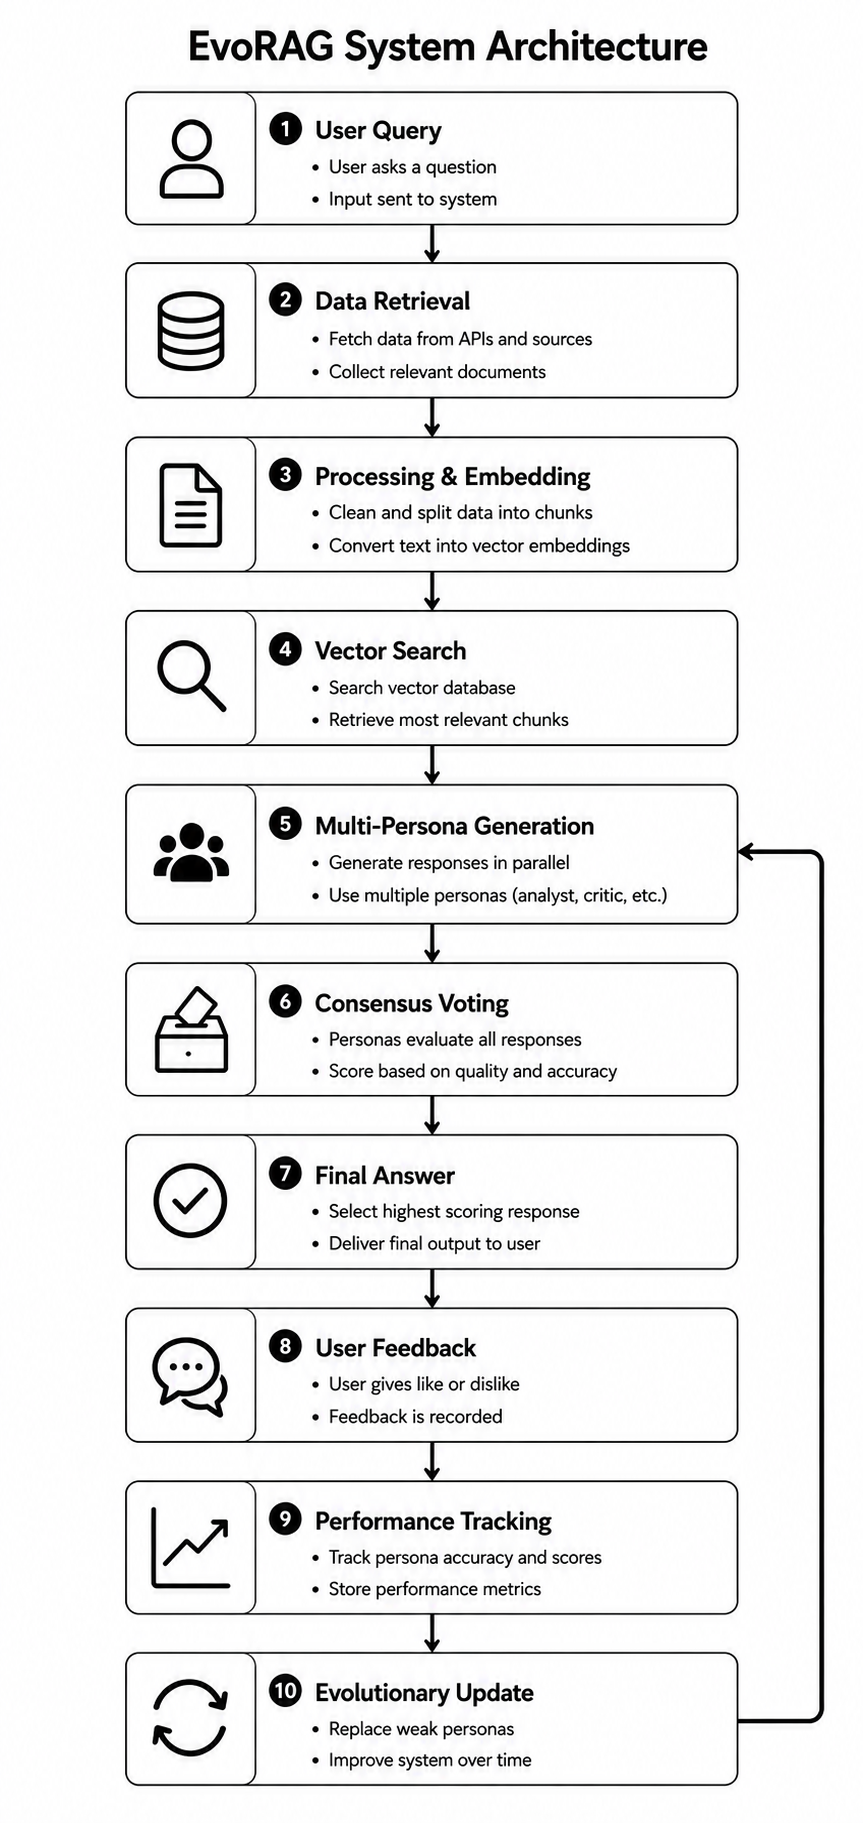
\includegraphics[width=0.70\linewidth]{Sys.png}
    \caption{EvoRAG System Architecture FlowChart}
    \label{fig:evorag_architecture}
\end{figure}

\begin{figure}[H]
    \centering
    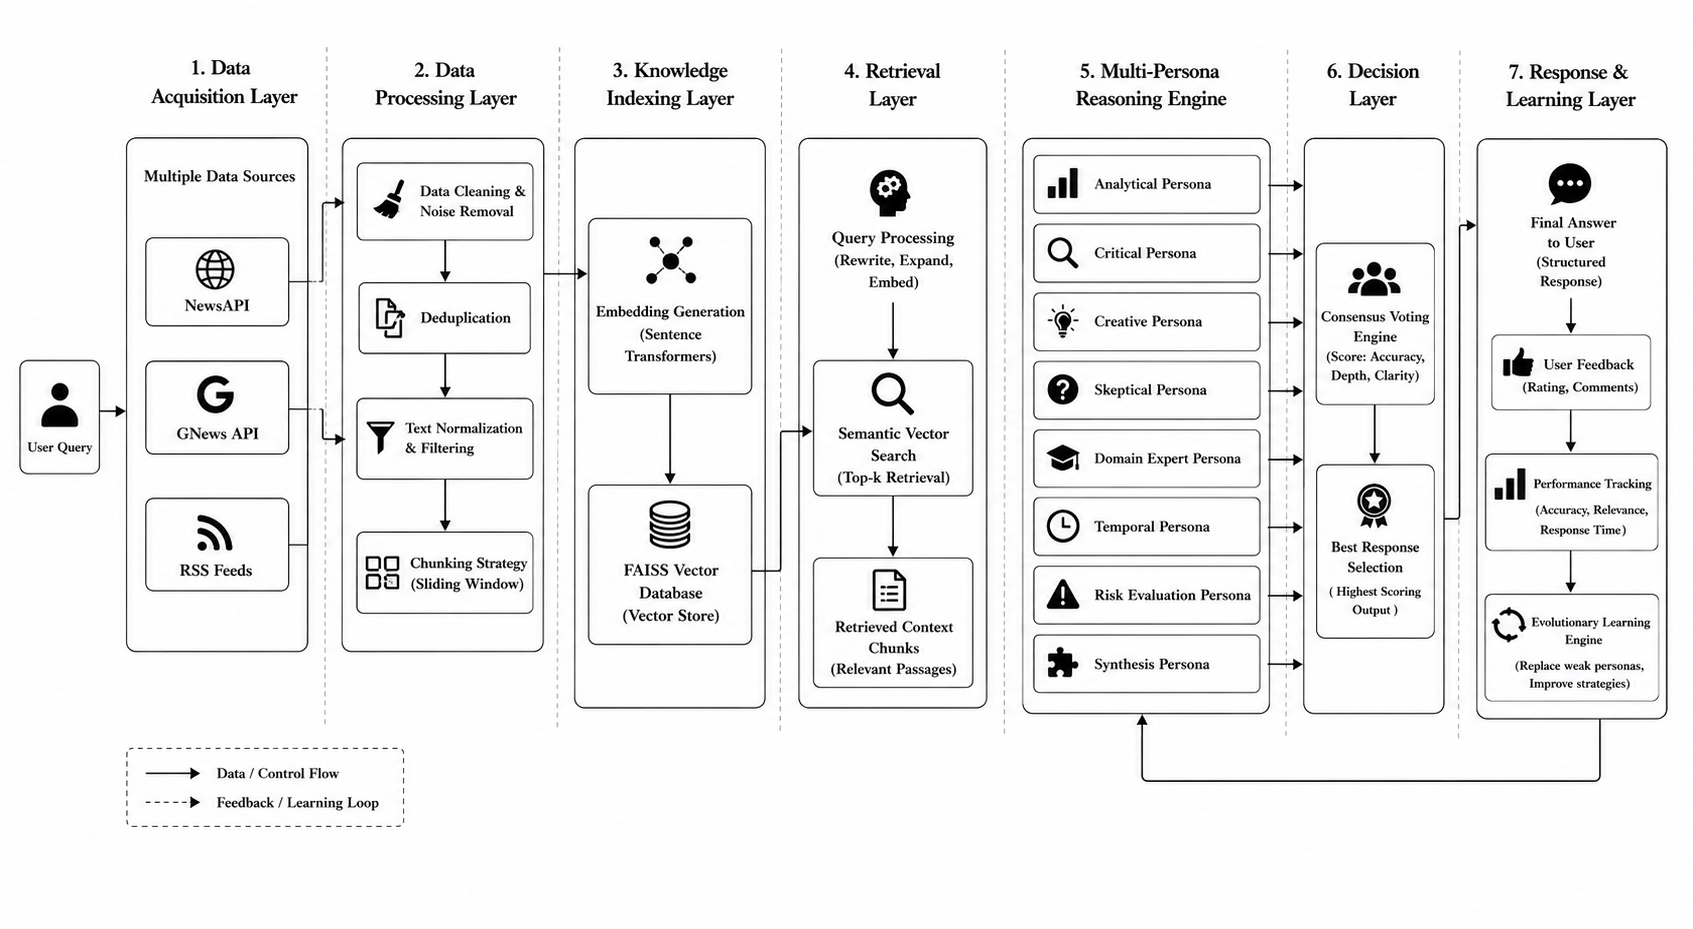
\includegraphics[width=0.95\linewidth]{sA2.png}
    \caption{EvoRAG System Architecture and Evolutionary Loop}
    \label{fig:evorag_architecture}
\end{figure}


\subsection{High Level Design}

The high level design illustrates the major modules of the EvoRAG system and their interactions.

\begin{figure}[H]
    \centering
    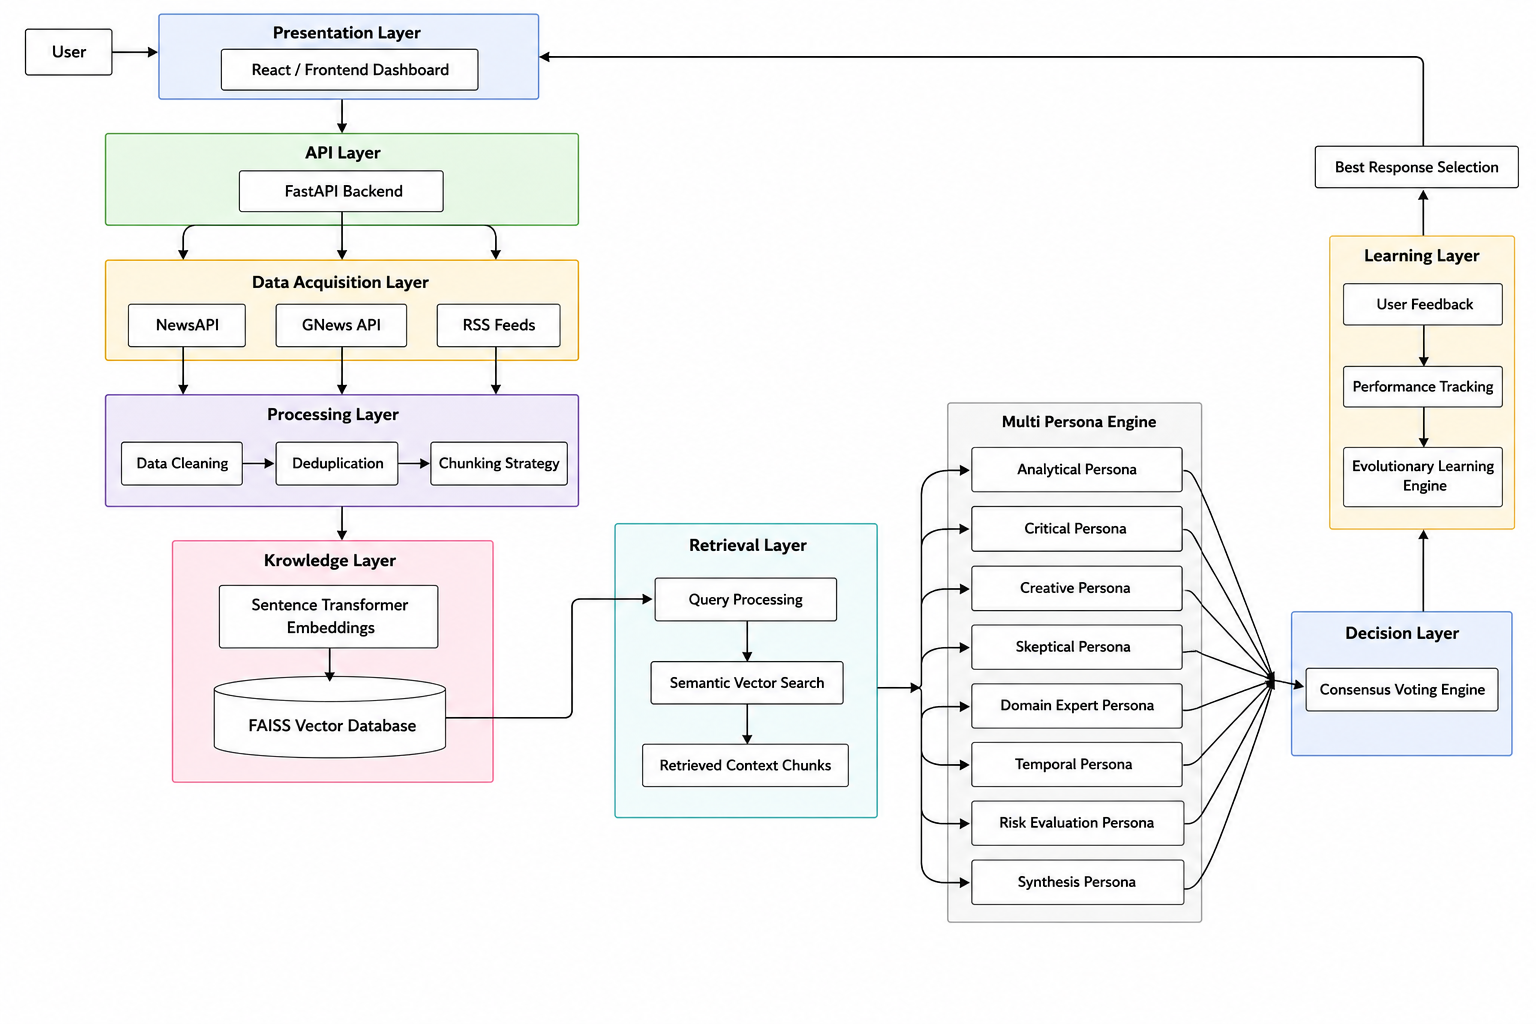
\includegraphics[width=0.85\linewidth,height=0.85\textheight,keepaspectratio]{hld.png}
    \caption{EvoRAG High Level Design}
    \label{fig:hld}
\end{figure}

\clearpage

\subsection{Low Level Design}

The low level design provides a detailed view of the internal logic within each
module, specifying the data flows, component interactions, API contracts, and
the sequence of operations that occur during a complete query-to-response cycle,
including the evolutionary feedback loop.

\begin{figure}[H]
    \centering
    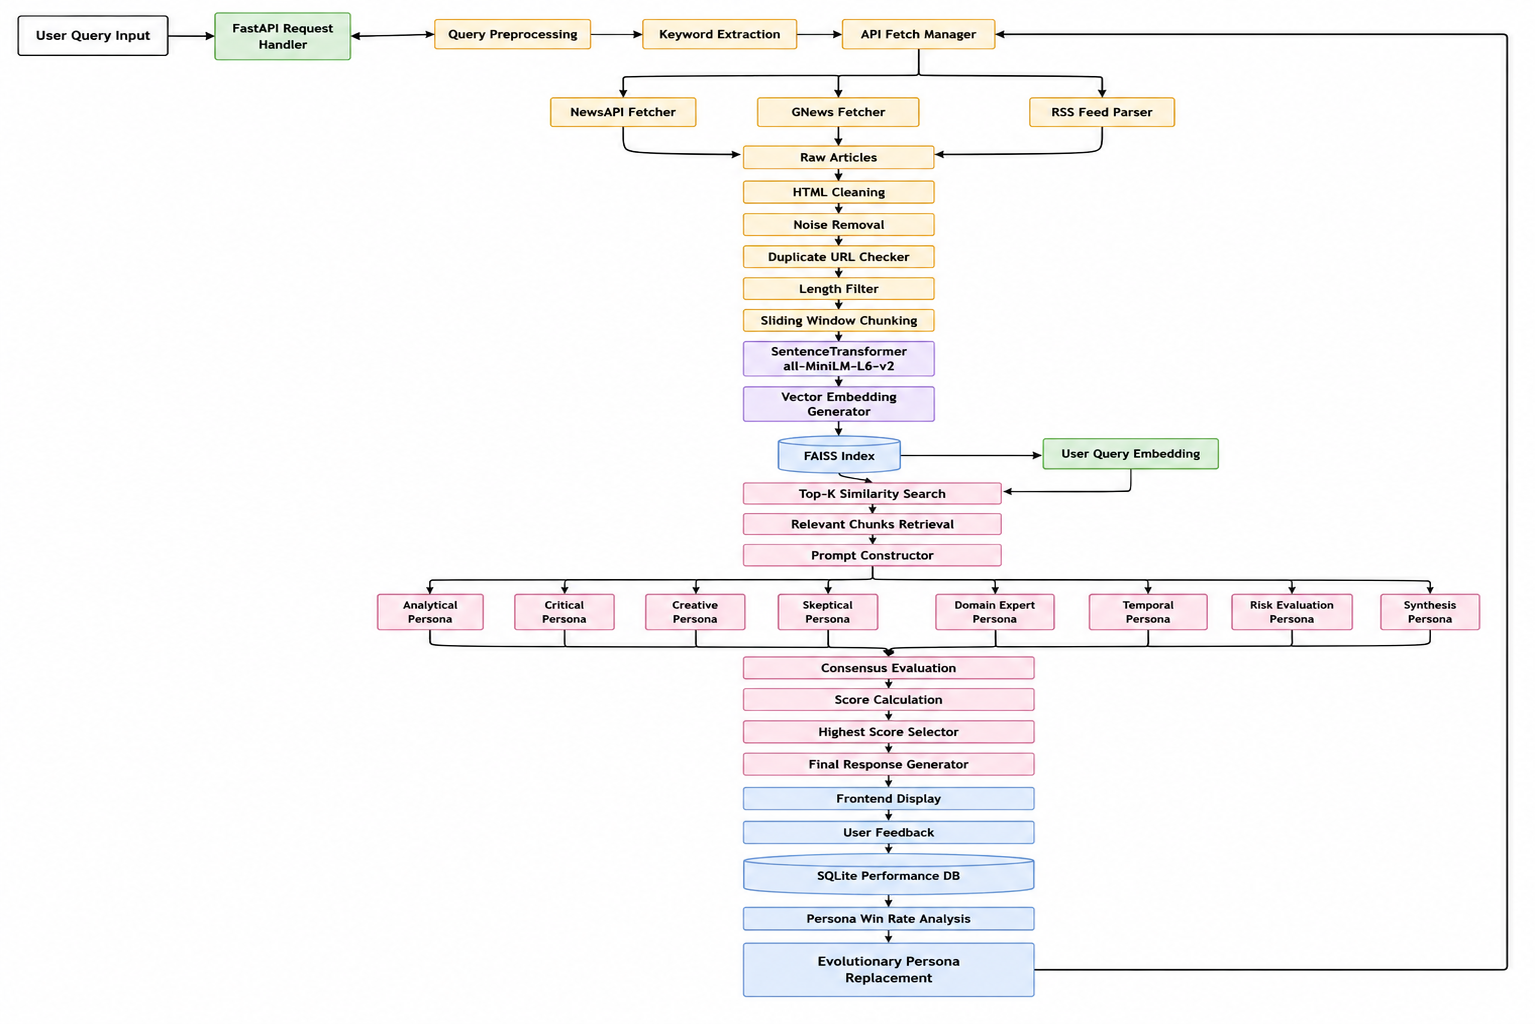
\includegraphics[width=\linewidth,height=\textheight,keepaspectratio]{lld2.png}
    \caption{EvoRAG Low Level Design}
    \label{fig:lld}
\end{figure}}

\chapter{Methodology}

\begin{figure}[H]
    \centering
    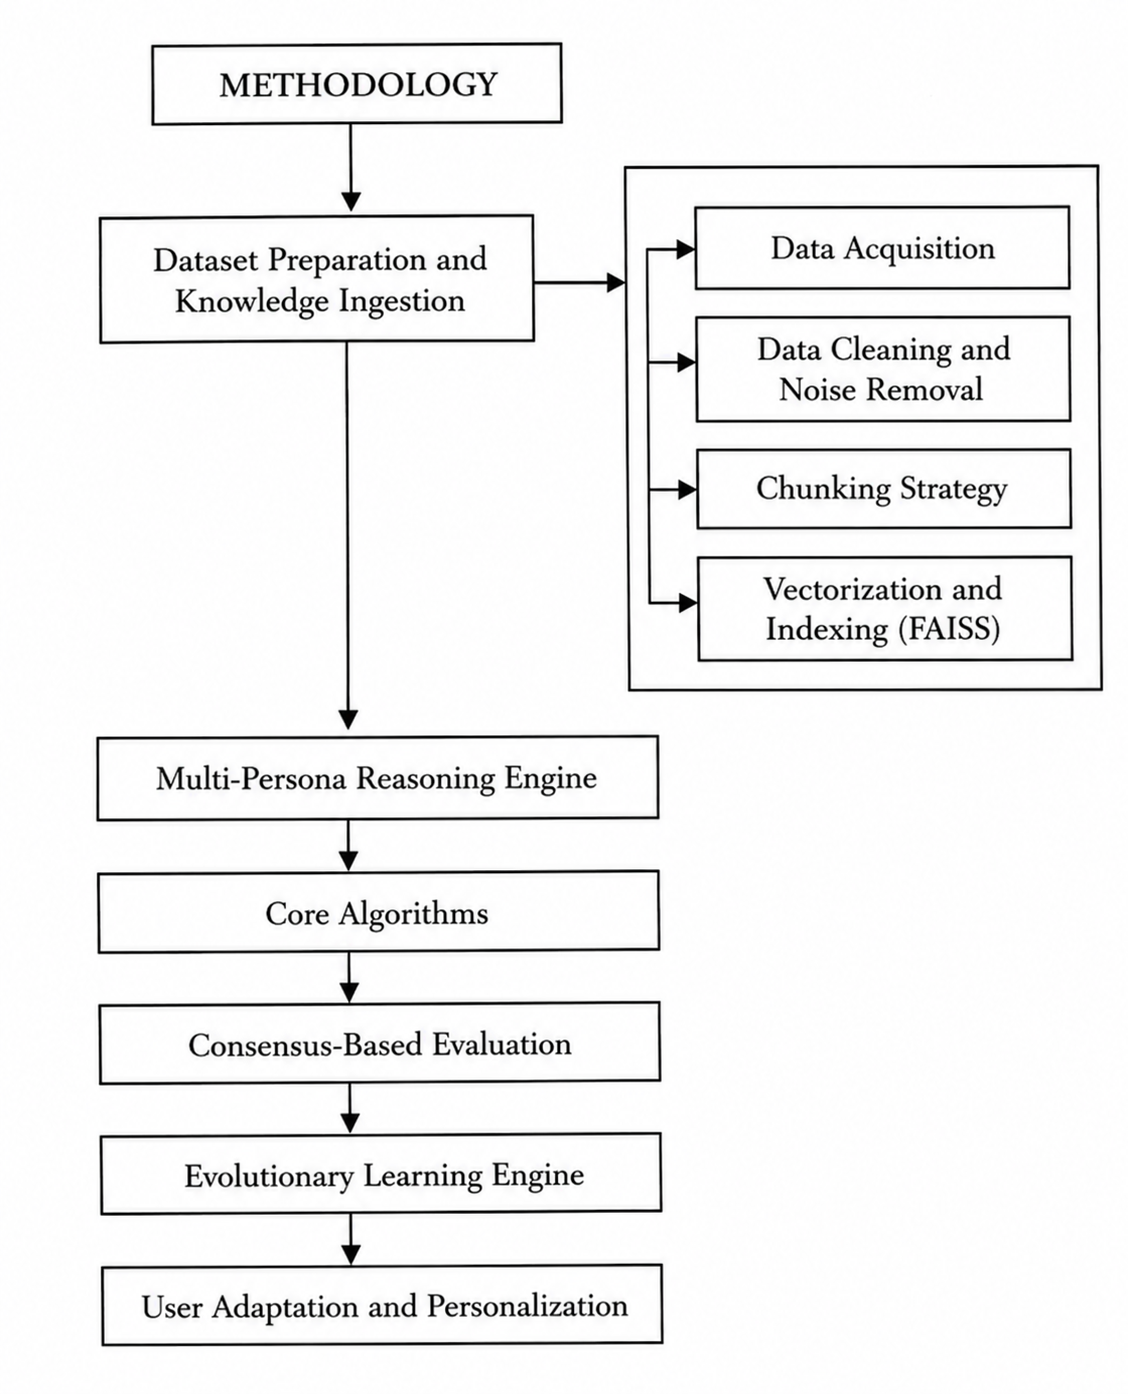
\includegraphics[width=0.75\linewidth]{method.png}
    \caption{EvoRAG Methodology Flowchart}
    \label{fig:method_flowchart}
\end{figure}

Figure~\ref{fig:method_flowchart} illustrates the complete EvoRAG methodology flow. The methodology of EvoRAG is divided into four core engines that work in tandem to produce high-quality, personalized results. It begins with dynamic data acquisition, progresses through data cleaning and chunking, indexes the resulting semantic vectors, and finishes with parallel multi-persona reasoning evaluated through consensus.

\section{Implementation}

This section explains the key implementation steps in the EvoRAG pipeline, covering data acquisition, cleaning, removal, chunking, indexing, and multi-persona reasoning.

\subsection{Data Acquisition}

The pipeline aggregates textual knowledge from three distinct live sources:

\begin{itemize}
    \item \textbf{NewsAPI:} Fetches comprehensive, real-time news articles from thousands of global publishers based on the user’s query keyword.
    \item \textbf{GNews API:} Retrieves top-ranking, highly credible articles indexed by Google News, providing broad topical coverage.
    \item \textbf{RSS Feeds:} Continuously monitored feeds from trusted, high-quality domains (e.g., BBC News, TechCrunch, Reuters) ensure a reliable baseline of verified journalism.
\end{itemize}

HTTP requests are handled via the \texttt{requests} library, while \texttt{feedparser} is used specifically for structured RSS feed parsing.

\subsection{Data Cleaning and Noise Removal}

Raw web content contains significant noise that must be eliminated before the data can be used for reasoning. The following cleaning steps are applied automatically:

\begin{itemize}
    \item \textbf{HTML Stripping:} The BeautifulSoup4 library parses each fetched page and removes all non-content elements including CSS stylesheets, JavaScript blocks, navigation menus, and advertisement banners, isolating only the pure article body text.
    \item \textbf{Deduplication:} Each article URL is hashed using SHA-256 before ingestion. Any URL whose hash already exists in the current session index is silently discarded, preventing the LLM from processing redundant or repeated information.
    \item \textbf{Length Filtering:} Articles falling below a minimum character threshold are discarded as they are unlikely to contain substantive analytical content.
\end{itemize}

\subsection{Chunking Strategy}

Large Language Models operate under strict context window and token limitations, making it impractical to feed entire articles as input. To address this, a sliding-window chunking strategy is applied.

\begin{itemize}
    \item \textbf{Chunk Size:} Each cleaned article is split into segments of approximately 300--400 words.
    \item \textbf{Overlap:} A 50-word overlap is maintained between consecutive chunks to ensure that contextual continuity across paragraph boundaries is preserved and no critical information is lost at chunk edges.
\end{itemize}

\subsection{Vectorization and Indexing (FAISS)}

Once chunked, the text segments are transformed into a machine-searchable vector database.

\begin{itemize}
    \item \textbf{Embedding Generation:} Each text chunk is passed through the \texttt{sentence-transformers} model (\texttt{all-MiniLM-L6-v2}), which encodes it into a high-dimensional dense vector representation capturing its semantic meaning.
    \item \textbf{FAISS Indexing:} All generated embeddings are stored in a local FAISS (Facebook AI Similarity Search) index using a flat L2 index structure that performs exact nearest-neighbour search, guaranteeing deterministic retrieval for identical query embeddings across sessions.
    \item \textbf{Metadata Preservation:} Alongside each embedding, the source URL, article title, and publication timestamp are stored as metadata to support source attribution in the final output.
\end{itemize}

This FAISS index constitutes the runtime dataset from which the multi-persona generation engine retrieves its grounding context.
At query time, the user's input is independently embedded using the same \texttt{all-MiniLM-L6-v2} model to produce a query vector, which is then compared against all stored chunk vectors to return the top-3 most semantically relevant passages as the retrieval context.
\subsection{Multi-Persona Reasoning Engine}

Instead of relying on a single output, EvoRAG employs a parallel generation strategy that produces eight independent analytical responses within a single LLM call.

\begin{itemize}
    \item \textbf{Structured Single-Call Generation:} The retrieved context and user query are packaged into a structured prompt that instructs the locally hosted Ollama LLM to simultaneously produce eight distinct persona responses in a single inference call, formatted as a parseable JSON object.
    \item \textbf{Diverse Personas:} Eight analytical personas — Analytical-Critical, Empirical-Evidential, Adversarial-Sceptical, Creative-Lateral, Domain-Expert, Temporal-Contextual, Risk-Evaluative, and Synthesis-Integrative — each produce an independent perspective grounded in the same retrieved context.
    \item \textbf{JSON Parsing and Validation:} The raw LLM output is parsed as a structured JSON object; each entry contains the persona name and its corresponding answer text, which are then passed directly to the peer-review scoring stage.
    \item \textbf{Goal:} To improve reasoning depth and eliminate the single-perspective bias inherent in standard RAG models, while maintaining full local execution without multiple sequential API calls.
\end{itemize}

\clearpage

\section{Core Algorithms}

The technical implementation of EvoRAG relies on several core algorithmic concepts,
with the primary orchestration handled by the EvoRAG Pipeline described below.

\subsubsection{Evolutionary Multi-Persona RAG Algorithm}

\vspace{0.5em}

\begin{algorithm}[H]
\caption{EvoRAG Pipeline --- Query to Consensus Response}
\small
\SetAlgoLined
\KwIn{$user\_query$}
\KwOut{$best\_persona,\ best\_answer,\ score\_breakdown,\ sources$}

\BlankLine
\tcp{Step 1: Retrieval}
$chunks \leftarrow \text{FAISS\_Retrieve}(user\_query,\ top\_k=3)$\;
\If{$chunks = \emptyset$}{
    \Return \textit{``No relevant context found.''}\;
}
$context \leftarrow \text{Merge}(chunks)$\;

\BlankLine
\tcp{Step 2: Multi-Persona Generation}
$personas \leftarrow \{$Analytical-Critical, Empirical-Evidential, Adversarial-Sceptical,
Creative-Lateral, Domain-Expert, Temporal-Contextual, Risk-Evaluative, Synthesis-Integrative$\}$\;
$prompt_{gen} \leftarrow \text{BuildPrompt}(user\_query,\ context,\ personas)$\;
$drafts \leftarrow \text{ParseJSON}(\text{LLM}(prompt_{gen}))$\;

\BlankLine
\tcp{Step 3: Peer-Review Scoring}
$prompt_{judge} \leftarrow \text{BuildJudgePrompt}(user\_query,\ drafts)$\;
$scores \leftarrow \text{ParseJSON}(\text{LLM}(prompt_{judge}))$\;
\tcp*[r]{Factual Grounding (0--10) + Analytical Depth (0--10) + Clarity (0--10) $= /30$}

\BlankLine
\tcp{Step 4: Consensus Selection}
$best\_persona \leftarrow \arg\max_{p \in personas}\ scores[p]$\;
$best\_answer \leftarrow drafts[best\_persona].answer$\;

\BlankLine
\tcp{Step 5: Output}
\Return $\{best\_persona,\ best\_answer,\ scores,\ chunks.metadata\}$\;
\end{algorithm}

\section{Consensus-Based Evaluation}

The system implements a self-regulating peer-review mechanism.

\begin{itemize}
    \item \textbf{Peer Voting Mechanism:} Each persona evaluates all generated responses, acting as a “judge” for others.
    
    \item \textbf{Scoring Criteria:} Responses are graded on three dimensions: Factual Grounding, Analytical Depth, and Clarity.
    
    \item \textbf{Final Selection:} The highest-scoring response, representing the consensus of the brainstorming session, is chosen as the final output.
\end{itemize}

\section{Evolutionary Learning Engine}

To ensure continuous improvement without retraining the base LLM, an evolutionary layer is added.

\begin{itemize}
    \item \textbf{Performance Tracking:} The win rates and qualitative scores of each persona are stored in a local SQLite database.
    
    \item \textbf{Adaptive Replacement:} Personas that consistently fail to win the peer-review or receive poor user feedback are periodically replaced with new persona variants.
    
    \item \textbf{Self-Improvement:} This allows the system to evolve its intellectual makeup over time based on the specific types of queries it receives.
\end{itemize}

\section{User Adaptation and Personalization}

The system adapts to individual user needs through a feedback loop.

\begin{itemize}
    \item \textbf{Feedback Integration:} The UI records user likes and dislikes for each response.
    
    \item \textbf{Affinity Modeling:} Personalized preference profiles are built, identifying which personas or response styles the user prefers.
    
    \item \textbf{Adaptive Output:} The voting weights in the consensus phase are dynamically adjusted based on these preference profiles.
\end{itemize}
%\input{results.tex}
\chapter{Conclusion}

\section{Overall Conclusion}

This project presents the design and partial implementation of \textbf{EvoRAG (Evolutionary Multi-Persona RAG)}, a locally deployed, multi-agent framework intended to improve the quality and reliability of retrieval-augmented generation. The core pipeline has been successfully implemented, covering the full flow from user query handling through to multi-persona response generation and consensus-based answer selection. The implemented stages demonstrate that structured cognitive diversity, applied to a retrieval pipeline, can produce more balanced and analytically grounded responses compared to standard single-pass RAG systems. While the system is not yet fully complete, the foundational components are functional and validate the core idea of the project.

\section{Summary of Work Done}

The current implementation covers the primary stages of the EvoRAG pipeline. The system is capable of accepting user queries, retrieving relevant information from external sources, and processing that information into searchable vector embeddings. Using semantic search, the most contextually relevant content is identified and passed to a set of eight AI personas, each of which independently generates a response based on its designated reasoning style. These responses are then evaluated through a consensus voting mechanism that scores each output for accuracy, depth, and clarity, and selects the most suitable response as the final answer. Together, these stages form a coherent and functional core pipeline that demonstrates the feasibility of the proposed approach.


% ------------------------------------------------------------------
%  BIBLIOGRAPHY
% ------------------------------------------------------------------
\addcontentsline{toc}{chapter}{Bibliography}
\begin{thebibliography}{99}
 
% [1]
\bibitem{lewis2020rag}
Patrick Lewis, Ethan Perez, Aleksandra Piktus, Fabio Petroni, Vladimir Karpukhin,
Naman Goyal, Heinrich K\"{u}ttler, Mike Lewis, Wen-tau Yih, Tim Rockt\"{a}schel,
Sebastian Riedel, and Douwe Kiela.
\newblock ``Retrieval-Augmented Generation for Knowledge-Intensive NLP Tasks,''
\newblock {\em Advances in Neural Information Processing Systems (NeurIPS)}, 2020.
 
% [2]
\bibitem{yao2022react}
Shunyu Yao, Jeffrey Zhao, Dian Yu, Nan Du, Izhak Shafran, Karthik Narasimhan,
and Yuan Cao.
\newblock ``ReAct: Synergizing Reasoning and Acting in Language Models,''
\newblock {\em arXiv preprint arXiv:2210.03629}, 2022.
 
% [3]
\bibitem{schick2023toolformer}
Timo Schick, Jane Dwivedi-Yu, Roberto Dessi, Roberta Raileanu, Maria Lomeli,
Luke Zettlemoyer, Nicola Cancedda, and Thomas Scialom.
\newblock ``Toolformer: Language Models Can Teach Themselves to Use Tools,''
\newblock {\em arXiv preprint arXiv:2302.04761}, 2023.
 
% [4]
\bibitem{asai2023selfrag}
Akari Asai, Zeqiu Wu, Yizhong Wang, Avirup Sil, and Hannaneh Hajishirzi.
\newblock ``Self-RAG: Learning to Retrieve, Generate, and Critique through
Self-Reflection,''
\newblock {\em arXiv preprint arXiv:2310.11511}, 2023.
 
% [5]
\bibitem{bommasani2021foundation}
Rishi Bommasani, Drew A. Hudson, Ehsan Adeli, Russ Altman, Simran Arora,
Sydney von Arx, Michael S. Bernstein, et al.
\newblock ``On the Opportunities and Risks of Foundation Models,''
\newblock {\em arXiv preprint arXiv:2108.07258}, 2021.
 
% [6]
\bibitem{singh2025agenticrag}
Aditi Singh, Abul Ehtesham, Saket Kumar, and Tala Talaei Khoei.
\newblock ``Agentic Retrieval-Augmented Generation: A Survey on Agentic RAG,''
\newblock {\em arXiv preprint arXiv:2501.09136}, 2025.
 
% [7]
\bibitem{du2026arag}
Mingxuan Du, Benfeng Xu, Chiwei Zhu, Shaohan Wang, Pengyu Wang, Xiaorui Wang,
and Zhendong Mao.
\newblock ``A-RAG: Scaling Agentic Retrieval-Augmented Generation via Hierarchical
Retrieval Interfaces,''
\newblock {\em arXiv preprint arXiv:2602.03442}, 2026.
 
% [8]
\bibitem{li2025ragreas}
Yangning Li et al.
\newblock ``Towards Agentic RAG with Deep Reasoning: A Survey of RAG-Reasoning
Systems in LLMs,''
\newblock {\em arXiv preprint arXiv:2507.09477}, 2025.
 
% [9]
\bibitem{sarthi2024raptor}
Parth Sarthi, Salman Abdullah, Aditi Tuli, Shubh Khanna, Anna Goldie,
and Christopher D. Manning.
\newblock ``RAPTOR: Recursive Abstractive Processing for Tree-Organized Retrieval,''
\newblock {\em arXiv preprint arXiv:2401.18059}, 2024.
 
% [10]
\bibitem{edge2024graphrag}
Darren Edge, Ha Trinh, Newman Cheng, Joshua Bradley, Alex Chao, Apurva Mody,
Steven Truitt, and Jonathan Larson.
\newblock ``From Local to Global: A Graph RAG Approach to Query-Focused
Summarization,''
\newblock {\em arXiv preprint arXiv:2404.16130}, 2024.
 
% [11]
\bibitem{pan2024unifying}
Shirui Pan, Linhao Luo, Yufei Wang, Chen Chen, Jiapu Wang, and Xindong Wu.
\newblock ``Unifying Large Language Models and Knowledge Graphs: A Roadmap,''
\newblock {\em IEEE Transactions on Knowledge and Data Engineering}, 2024.
 
% [12]
\bibitem{manakul2023selfcheckgpt}
Potsawee Manakul, Adian Liusie, and Mark J. F. Gales.
\newblock ``SelfCheckGPT: Zero-Resource Black-Box Hallucination Detection for
Generative Large Language Models,''
\newblock {\em arXiv preprint arXiv:2303.08896}, 2023.
 
% [13]
\bibitem{mallen2023trust}
Alex Mallen, Akari Asai, Victor Zhong, Rajarshi Das, Daniel Khashabi,
and Hannaneh Hajishirzi.
\newblock ``When Not to Trust Language Models: Investigating Effectiveness of
Parametric and Non-Parametric Memories,''
\newblock {\em Proceedings of the 61st Annual Meeting of the Association for
Computational Linguistics (ACL)}, 2023.
 
% [14]
\bibitem{shi2023replug}
Weijia Shi, Sewon Min, Michihiro Yasunaga, Minjoon Seo, Rich James,
Mike Lewis, Luke Zettlemoyer, and Wen-tau Yih.
\newblock ``REPLUG: Retrieval-Augmented Black-Box Language Models,''
\newblock {\em arXiv preprint arXiv:2301.12652}, 2023.
 
% [15]
\bibitem{nguyen2025marag}
Thang Nguyen, Peter Chin, and Yu-Wing Tai.
\newblock ``MA-RAG: Multi-Agent Retrieval-Augmented Generation via Collaborative
Chain-of-Thought Reasoning,''
\newblock {\em arXiv preprint arXiv:2505.20096}, 2025.
 
% [16]
\bibitem{xiao2026massrag}
Xingchen Xiao et al.
\newblock ``MASS-RAG: Multi-Agent Synthesis Retrieval-Augmented Generation,''
\newblock {\em arXiv preprint arXiv:2604.18509}, 2026.
 
% [17]
\bibitem{xu2026anchorrag}
Jiasheng Xu, Mingda Li, Yongqiang Tang, Peijie Wang, and Wensheng Zhang.
\newblock ``Towards Open-World Retrieval-Augmented Generation on Knowledge Graph:
A Multi-Agent Collaboration Framework,''
\newblock {\em Proceedings of the ACM Web Conference (WWW~'26)}, 2026.
 
% [18]
\bibitem{zheng2025deepdx}
Qiaoyu Zheng et al.
\newblock ``End-to-End Agentic RAG System Training for Traceable Diagnostic
Reasoning,''
\newblock {\em arXiv preprint arXiv:2508.15746}, 2025.
 
% [19]
\bibitem{ouyang2022rlhf}
Long Ouyang, Jeffrey Wu, Xu Jiang, Diogo Almeida, Carroll Wainwright,
Pamela Mishkin, Chong Zhang, Sandhini Agarwal, Katarina Slama, Alex Ray,
John Schulman, Jacob Hilton, Fraser Kelton, Luke Miller, Maddie Simens,
Amanda Askell, Peter Welinder, Paul Christiano, Jan Leike, and Ryan Lowe.
\newblock ``Training Language Models to Follow Instructions with Human Feedback,''
\newblock {\em Advances in Neural Information Processing Systems (NeurIPS)}, 2022.
 
% [20]
\bibitem{anonymous2026ragshaper}
Anonymous.
\newblock ``RAGShaper: Eliciting Sophisticated Agentic RAG Skills via Automated
Data Synthesis,''
\newblock {\em arXiv preprint arXiv:2601.08699}, 2026.
 
% [21]
\bibitem{izacard2022atlas}
Gautier Izacard, Patrick Lewis, Maria Lomeli, Lucas Hosseini, Fabio Petroni,
Timo Schick, Jane Dwivedi-Yu, Armand Joulin, Sebastian Riedel, and Edouard Grave.
\newblock ``Atlas: Few-Shot Learning with Retrieval Augmented Language Models,''
\newblock {\em Journal of Machine Learning Research (JMLR)}, vol.~24, 2023.
 
% [22]
\bibitem{hu2025memory}
Yuyang Hu, Shichun Liu, Yanwei Yue, Guibin Zhang, et al.
\newblock ``Memory in the Age of AI Agents,''
\newblock {\em arXiv preprint arXiv:2512.13564}, 2025.
 
% [23]
\bibitem{chen2026agemem}
Xiangyu Chen et al.
\newblock ``Agentic Memory: Learning Unified Long-Term and Short-Term Memory
Management for Large Language Model Agents,''
\newblock {\em arXiv preprint arXiv:2601.01885}, 2026.
 
% [24]
\bibitem{bai2025memos}
Ting Bai et al.
\newblock ``Memory OS of AI Agent,''
\newblock {\em arXiv preprint arXiv:2506.06326}, 2025.
 
% [25]
\bibitem{besrour2026agenticvsenh}
Ines Besrour et al.
\newblock ``Is Agentic RAG Worth It? An Experimental Comparison of RAG Approaches,''
\newblock {\em arXiv preprint arXiv:2601.07711}, 2026.
 
% [26]
\bibitem{gan2025rageval}
Aoran Gan et al.
\newblock ``Retrieval Augmented Generation Evaluation in the Era of Large Language
Models: A Comprehensive Survey,''
\newblock {\em arXiv preprint arXiv:2504.14891}, 2025.
 
% [27]
\bibitem{guu2020realm}
Kelvin Guu, Kenton Lee, Zora Tung, Panupong Pasupat, and Ming-Wei Chang.
\newblock ``REALM: Retrieval-Augmented Language Model Pre-Training,''
\newblock {\em International Conference on Machine Learning (ICML)}, 2020.
 
% [28]
\bibitem{izacard2021passage}
Gautier Izacard and Edouard Grave.
\newblock ``Leveraging Passage Retrieval with Generative Models for Open Domain
Question Answering,''
\newblock {\em arXiv preprint arXiv:2007.01282}, 2021.
 
% [29]
\bibitem{wei2022cot}
Jason Wei, Xuezhi Wang, Dale Schuurmans, Maarten Bosma, Brian Ichter,
Fei Xia, Ed Chi, Quoc Le, and Denny Zhou.
\newblock ``Chain-of-Thought Prompting Elicits Reasoning in Large Language Models,''
\newblock {\em Advances in Neural Information Processing Systems (NeurIPS)}, 2022.
 
% [30]
\bibitem{gao2023ragsurvey}
Yunfan Gao, Yun Xiong, Xinyu Gao, Kangxiang Jia, Jinliu Pan, Yuxi Bi,
Yi Dai, Jiawei Sun, and Haofen Wang.
\newblock ``Retrieval-Augmented Generation for Large Language Models: A Survey,''
\newblock {\em arXiv preprint arXiv:2312.10997}, 2023.
 
\end{thebibliography}
\begin{appendices}

% =========================================================
% APPENDIX A
% =========================================================

\chapter{Project Planning}

% ---------------------------------------------------------
\section{Project Timeline}

The EvoRAG project development was initiated during Semester VI following the project timeline illustrated in Figure A.1. 
The completed work in this phase includes problem identification, literature survey, requirement analysis, system architecture design, and initial implementation of the retrieval and multi-persona reasoning modules. 
Further development, testing, optimization, dashboard integration, and final deployment will be continued in the upcoming semester.

\vspace{0.5cm}

\begin{figure}[H]
    \centering
    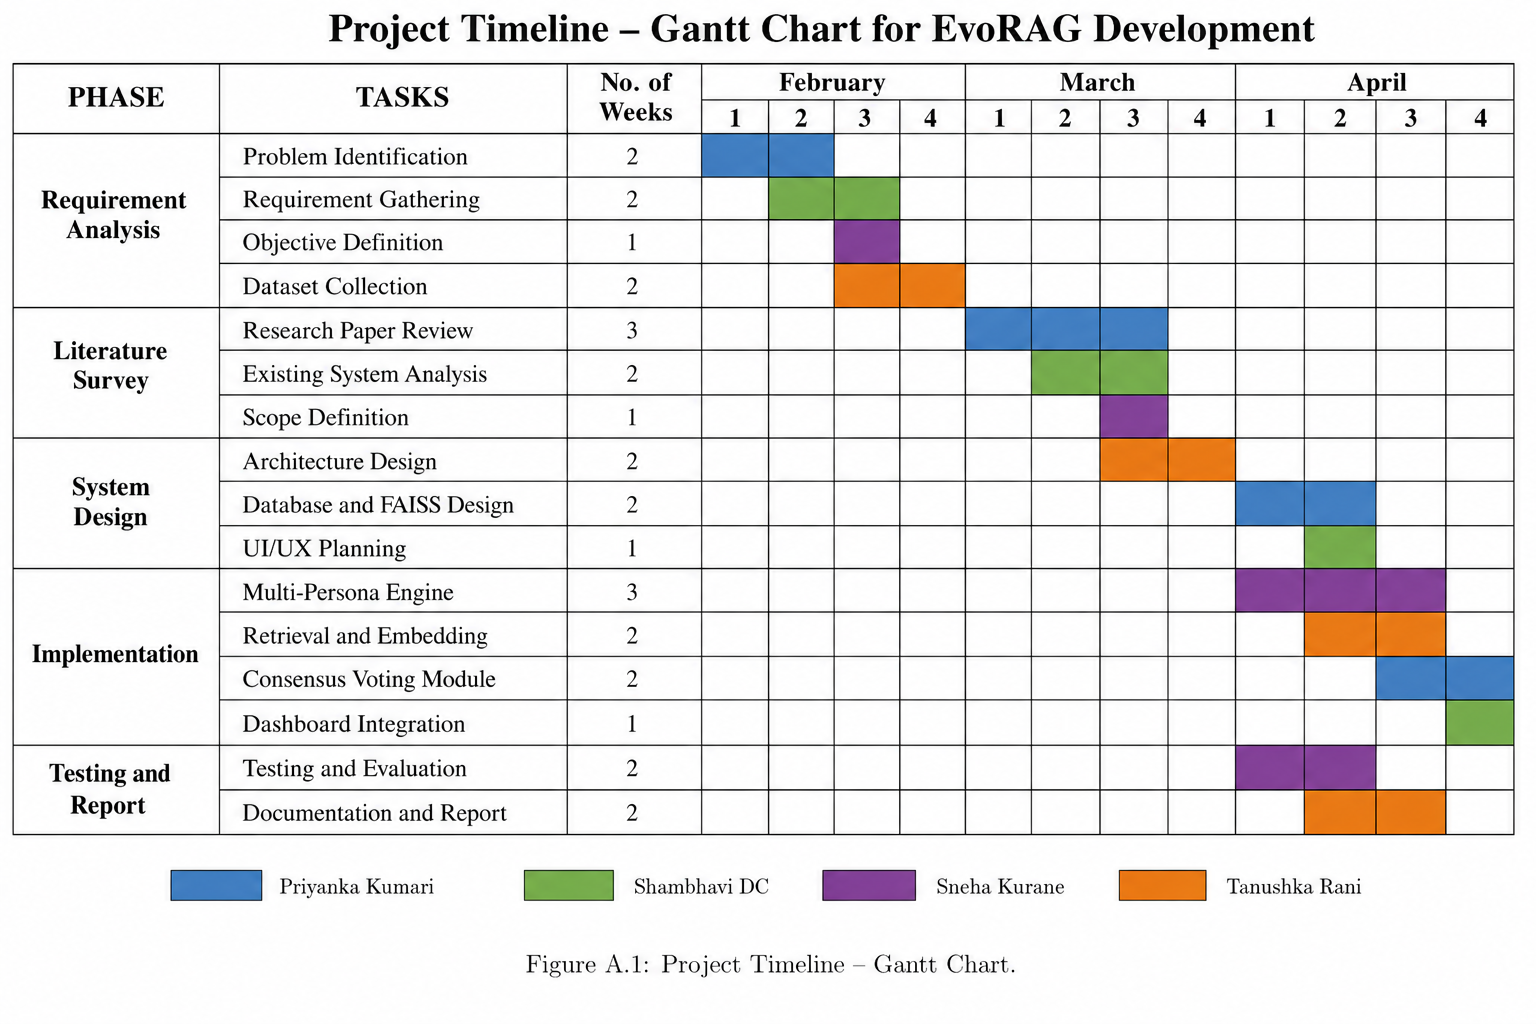
\includegraphics[width=\linewidth]{timeline.png}
    \caption{Project Timeline -- Gantt Chart}
    \label{fig:timeline}
\end{figure}

\clearpage

% ---------------------------------------------------------
\section{Budget Estimation}

This section presents the estimated budget required for the development and deployment of the EvoRAG system. 
The budget mainly includes software tools, API usage, cloud resources, development infrastructure, and miscellaneous expenses incurred during the project implementation.

\vspace{0.5cm}

\begin{table}[H]
\centering
\renewcommand{\arraystretch}{1.3}

\begin{tabular}{|c|p{8cm}|c|}
\hline

\textbf{SL. NO.} &
\centering \textbf{Software / Resources} &
\textbf{Estimated Cost [INR]}
\tabularnewline

\hline

1 & Development System and Internet Resources & 15,000 \\
\hline

2 & NewsAPI Subscription / API Usage & 2,000 \\
\hline

3 & GNews API and RSS Feed Integration & 1,500 \\
\hline

4 & Python Libraries and Development Tools & 0 (Open Source) \\
\hline

5 & FAISS Vector Database Setup & 0 (Open Source) \\
\hline

6 & Sentence Transformer Models & 0 (Open Source) \\
\hline

7 & Local LLM Deployment and Testing & 3,000 \\
\hline

8 & Frontend Dashboard Development & 2,500 \\
\hline

9 & Testing, Evaluation and Documentation & 2,000 \\
\hline

10 & Miscellaneous Expenses & 1,500 \\
\hline

\multicolumn{2}{|c|}{\textbf{Total Estimated Cost}} &
\textbf{27,500 INR} \\
\hline

\end{tabular}

\vspace{0.5cm}

\caption{Budget Estimation for the EvoRAG Project}
\label{tab:budget_estimation}

\end{table}

% =========================================================
% APPENDIX B
% =========================================================

\chapter{Dataset and Input Details}

The EvoRAG system utilizes a dynamic knowledge ingestion pipeline to ensure that retrieved information remains current, reliable, and contextually relevant for every user query. 
The dataset is generated dynamically at runtime using multiple live data sources instead of relying on static pre-trained corpora.

The system gathers information from APIs such as NewsAPI and GNews API along with trusted RSS feeds. 
The collected data undergoes cleaning, deduplication, chunking, and embedding generation before being stored in a FAISS vector database for semantic retrieval.

The input pipeline supports:
\begin{itemize}
    \item Real-time query-based data collection
    \item Data cleaning using BeautifulSoup
    \item Sliding-window chunking strategy
    \item Embedding generation using sentence-transformers
    \item Efficient vector search using FAISS indexing
\end{itemize}

% =========================================================
% APPENDIX C
% =========================================================

\chapter{Configuration Details}

This appendix provides the technical configuration and environment details required to execute the EvoRAG system efficiently.

The project was developed using Python and integrated with various libraries and frameworks for vector retrieval, multi-persona reasoning, and dashboard visualization.

\textbf{Hardware Requirements}
\begin{itemize}
    \item Intel Core i7 / AMD Ryzen 7 Processor
    \item Minimum 16GB RAM
    \item SSD Storage
    \item NVIDIA GPU (recommended for faster inference)
\end{itemize}

\textbf{Software Requirements}
\begin{itemize}
    \item Python 3.10+
    \item FAISS Vector Database
    \item LangChain Framework
    \item Ollama for Local LLM Execution
    \item BeautifulSoup4 and Pandas
    \item SQLite Database
\end{itemize}

\textbf{Environment Setup}
\begin{enumerate}
    \item Clone the repository: \texttt{git clone https://github.com/prowessclust/evorag}
    \item Create a virtual environment: \texttt{python -m venv venv}
    \item Activate the environment and install dependencies: \texttt{pip install -r requirements.txt}
    \item Configure the local LLM via Ollama: \texttt{ollama pull mistral} or \texttt{ollama pull llama3}
\end{enumerate}

\textbf{Project Repository}

The complete project source code and implementation details are maintained in the GitHub repository.

\begin{center}
\url{https://github.com/prowessclust/evorag}
\end{center}

\end{appendices}
 

\end{document}

